% Options for packages loaded elsewhere
\PassOptionsToPackage{unicode}{hyperref}
\PassOptionsToPackage{hyphens}{url}
\PassOptionsToPackage{dvipsnames,svgnames,x11names}{xcolor}
\documentclass[
  10pt,
]{article}
\usepackage{xcolor}
\usepackage{amsmath,amssymb}
\setcounter{secnumdepth}{-\maxdimen} % remove section numbering
\usepackage{iftex}
\ifPDFTeX
  \usepackage[T1]{fontenc}
  \usepackage[utf8]{inputenc}
  \usepackage{textcomp} % provide euro and other symbols
\else % if luatex or xetex
  \usepackage{unicode-math} % this also loads fontspec
  \defaultfontfeatures{Scale=MatchLowercase}
  \defaultfontfeatures[\rmfamily]{Ligatures=TeX,Scale=1}
\fi
\usepackage{lmodern}
\ifPDFTeX\else
  % xetex/luatex font selection
\fi
% Use upquote if available, for straight quotes in verbatim environments
\IfFileExists{upquote.sty}{\usepackage{upquote}}{}
\IfFileExists{microtype.sty}{% use microtype if available
  \usepackage[]{microtype}
  \UseMicrotypeSet[protrusion]{basicmath} % disable protrusion for tt fonts
}{}
\makeatletter
\@ifundefined{KOMAClassName}{% if non-KOMA class
  \IfFileExists{parskip.sty}{%
    \usepackage{parskip}
  }{% else
    \setlength{\parindent}{0pt}
    \setlength{\parskip}{6pt plus 2pt minus 1pt}}
}{% if KOMA class
  \KOMAoptions{parskip=half}}
\makeatother
\usepackage{color}
\usepackage{fancyvrb}
\newcommand{\VerbBar}{|}
\newcommand{\VERB}{\Verb[commandchars=\\\{\}]}
\DefineVerbatimEnvironment{Highlighting}{Verbatim}{commandchars=\\\{\}}
% Add ',fontsize=\small' for more characters per line
\newenvironment{Shaded}{}{}
\newcommand{\AlertTok}[1]{\textcolor[rgb]{1.00,0.00,0.00}{\textbf{#1}}}
\newcommand{\AnnotationTok}[1]{\textcolor[rgb]{0.38,0.63,0.69}{\textbf{\textit{#1}}}}
\newcommand{\AttributeTok}[1]{\textcolor[rgb]{0.49,0.56,0.16}{#1}}
\newcommand{\BaseNTok}[1]{\textcolor[rgb]{0.25,0.63,0.44}{#1}}
\newcommand{\BuiltInTok}[1]{\textcolor[rgb]{0.00,0.50,0.00}{#1}}
\newcommand{\CharTok}[1]{\textcolor[rgb]{0.25,0.44,0.63}{#1}}
\newcommand{\CommentTok}[1]{\textcolor[rgb]{0.38,0.63,0.69}{\textit{#1}}}
\newcommand{\CommentVarTok}[1]{\textcolor[rgb]{0.38,0.63,0.69}{\textbf{\textit{#1}}}}
\newcommand{\ConstantTok}[1]{\textcolor[rgb]{0.53,0.00,0.00}{#1}}
\newcommand{\ControlFlowTok}[1]{\textcolor[rgb]{0.00,0.44,0.13}{\textbf{#1}}}
\newcommand{\DataTypeTok}[1]{\textcolor[rgb]{0.56,0.13,0.00}{#1}}
\newcommand{\DecValTok}[1]{\textcolor[rgb]{0.25,0.63,0.44}{#1}}
\newcommand{\DocumentationTok}[1]{\textcolor[rgb]{0.73,0.13,0.13}{\textit{#1}}}
\newcommand{\ErrorTok}[1]{\textcolor[rgb]{1.00,0.00,0.00}{\textbf{#1}}}
\newcommand{\ExtensionTok}[1]{#1}
\newcommand{\FloatTok}[1]{\textcolor[rgb]{0.25,0.63,0.44}{#1}}
\newcommand{\FunctionTok}[1]{\textcolor[rgb]{0.02,0.16,0.49}{#1}}
\newcommand{\ImportTok}[1]{\textcolor[rgb]{0.00,0.50,0.00}{\textbf{#1}}}
\newcommand{\InformationTok}[1]{\textcolor[rgb]{0.38,0.63,0.69}{\textbf{\textit{#1}}}}
\newcommand{\KeywordTok}[1]{\textcolor[rgb]{0.00,0.44,0.13}{\textbf{#1}}}
\newcommand{\NormalTok}[1]{#1}
\newcommand{\OperatorTok}[1]{\textcolor[rgb]{0.40,0.40,0.40}{#1}}
\newcommand{\OtherTok}[1]{\textcolor[rgb]{0.00,0.44,0.13}{#1}}
\newcommand{\PreprocessorTok}[1]{\textcolor[rgb]{0.74,0.48,0.00}{#1}}
\newcommand{\RegionMarkerTok}[1]{#1}
\newcommand{\SpecialCharTok}[1]{\textcolor[rgb]{0.25,0.44,0.63}{#1}}
\newcommand{\SpecialStringTok}[1]{\textcolor[rgb]{0.73,0.40,0.53}{#1}}
\newcommand{\StringTok}[1]{\textcolor[rgb]{0.25,0.44,0.63}{#1}}
\newcommand{\VariableTok}[1]{\textcolor[rgb]{0.10,0.09,0.49}{#1}}
\newcommand{\VerbatimStringTok}[1]{\textcolor[rgb]{0.25,0.44,0.63}{#1}}
\newcommand{\WarningTok}[1]{\textcolor[rgb]{0.38,0.63,0.69}{\textbf{\textit{#1}}}}
\usepackage{longtable,booktabs,array}
\newcounter{none} % for unnumbered tables
\usepackage{calc} % for calculating minipage widths
% Correct order of tables after \paragraph or \subparagraph
\usepackage{etoolbox}
\makeatletter
\patchcmd\longtable{\par}{\if@noskipsec\mbox{}\fi\par}{}{}
\makeatother
% Allow footnotes in longtable head/foot
\IfFileExists{footnotehyper.sty}{\usepackage{footnotehyper}}{\usepackage{footnote}}
\makesavenoteenv{longtable}
% definitions for citeproc citations
\NewDocumentCommand\citeproctext{}{}
\NewDocumentCommand\citeproc{mm}{%
  \begingroup\def\citeproctext{#2}\cite{#1}\endgroup}
\makeatletter
 % allow citations to break across lines
 \let\@cite@ofmt\@firstofone
 % avoid brackets around text for \cite:
 \def\@biblabel#1{}
 \def\@cite#1#2{{#1\if@tempswa , #2\fi}}
\makeatother
\newlength{\cslhangindent}
\setlength{\cslhangindent}{1.5em}
\newlength{\csllabelwidth}
\setlength{\csllabelwidth}{3em}
\newenvironment{CSLReferences}[2] % #1 hanging-indent, #2 entry-spacing
 {\begin{list}{}{%
  \setlength{\itemindent}{0pt}
  \setlength{\leftmargin}{0pt}
  \setlength{\parsep}{0pt}
  % turn on hanging indent if param 1 is 1
  \ifodd #1
   \setlength{\leftmargin}{\cslhangindent}
   \setlength{\itemindent}{-1\cslhangindent}
  \fi
  % set entry spacing
  \setlength{\itemsep}{#2\baselineskip}}}
 {\end{list}}
\usepackage{calc}
\newcommand{\CSLBlock}[1]{\hfill\break\parbox[t]{\linewidth}{\strut\ignorespaces#1\strut}}
\newcommand{\CSLLeftMargin}[1]{\parbox[t]{\csllabelwidth}{\strut#1\strut}}
\newcommand{\CSLRightInline}[1]{\parbox[t]{\linewidth - \csllabelwidth}{\strut#1\strut}}
\newcommand{\CSLIndent}[1]{\hspace{\cslhangindent}#1}
\setlength{\emergencystretch}{3em} % prevent overfull lines
\providecommand{\tightlist}{%
  \setlength{\itemsep}{0pt}\setlength{\parskip}{0pt}}
% Extra preamble: Unicode characters used in the report body that plain
% pdflatex + inputenc(utf8)/fontenc(T1) do not already cover.
\DeclareUnicodeCharacter{0394}{\ensuremath{\Delta}}     % Δ
\DeclareUnicodeCharacter{03C0}{\ensuremath{\pi}}        % π
\DeclareUnicodeCharacter{03C1}{\ensuremath{\rho}}       % ρ
\DeclareUnicodeCharacter{03C9}{\ensuremath{\omega}}     % ω
\DeclareUnicodeCharacter{2191}{\ensuremath{\uparrow}}   % ↑
\DeclareUnicodeCharacter{2192}{\ensuremath{\rightarrow}}% →
\DeclareUnicodeCharacter{2193}{\ensuremath{\downarrow}} % ↓
\DeclareUnicodeCharacter{2208}{\ensuremath{\in}}        % ∈
\DeclareUnicodeCharacter{2212}{\ensuremath{-}}          % − (minus sign)
\DeclareUnicodeCharacter{2213}{\ensuremath{\mp}}        % ∓
\DeclareUnicodeCharacter{2248}{\ensuremath{\approx}}    % ≈
\DeclareUnicodeCharacter{2264}{\ensuremath{\leq}}       % ≤
\DeclareUnicodeCharacter{2265}{\ensuremath{\geq}}       % ≥

% Tables in the report are wider than the 1in-margin textwidth in places;
% allow small tables to shrink to fit rather than overflow.
\usepackage{adjustbox}

% Long inline results/*.json paths in \texttt{} (Appendix C/D/E artifact
% lists) have no natural break point; allow breaking at underscores/hyphens
% so they wrap instead of overflowing the margin.
\usepackage[htt]{hyphenat}

% Long, evidence-heavy paragraphs run pages before the next figure; keep
% figures near their reference point without forcing a hard float barrier.
\usepackage{float}

% [H] forces a figure to its exact source position even when it doesn't fit
% on the current page, leaving a large blank gap instead of flowing text
% around it. placeins' \FloatBarrier lets a figure float naturally ([htbp])
% while still forbidding it from drifting past a given point (e.g. past its
% own section), avoiding both the drift and the forced-gap failure modes.
\usepackage{placeins}

% Appendix A's verbatim prompt text has long lines; pandoc's fenced-code
% Highlighting environment (fancyvrb Verbatim) doesn't wrap by default,
% which overflows the page margin. Wrap and shrink it slightly instead.
\usepackage{fvextra}
\DefineVerbatimEnvironment{Highlighting}{Verbatim}{commandchars=\\\{\},breaklines=true,breakanywhere=true,fontsize=\small}

% Bullets (e.g. the metric definitions in 3.4) often contain long inline
% `code` spans -- pandoc renders their internal spaces as fixed-width \
% control spaces, so the whole span is one unbreakable chunk near a full
% line's width. Under full justification, LaTeX compensates by stretching
% the few remaining breakable spaces on that line unevenly. Ragged-right
% itemize lets the leftover space fall to the margin instead.
\AtBeginEnvironment{itemize}{\raggedright}
% Loaded after report/latex/preamble.tex (and after pandoc's own font setup) so
% that neurips_2026.sty's Times/Helvetica selection and its \newgeometry (set in
% \AtBeginDocument) win over pandoc's defaults, mirroring the load-order logic
% the arXiv build uses for arxiv.sty.
%
% Options:
%   dblblindworkshop -- the Workshop / double-blind reviewing track. Keeps
%                       \if@anonymous true (so \@maketitle prints "Anonymous
%                       Author(s)" and ignores \@author entirely) and, in
%                       camera-ready mode, prints \workshoptitle in the notice.
%   nonatbib         -- pandoc renders the bibliography via citeproc (a CSL
%                       reference list in the body), so natbib is unused; not
%                       loading it avoids any clash with pandoc's hyperref.
\usepackage[final,nonatbib]{neurips_2026}
\makeatletter
\renewcommand{\@noticestring}{Workshop on Who Verifies the Agents? Toward Reliable Agent Development, NeurIPS 2026.}
\makeatother

% neurips_2026.sty sets \flushbottom, which combined with pandoc's stretchy
% \parskip stretches interline space to fill short pages exactly, producing
% large visible gaps around figures on pages with few paragraphs. Same override
% the arXiv build applies for the same reason.
\raggedbottom

% The 5.5in block is narrower than the arXiv build's, so a few of the long
% inline \texttt{} spans (model snapshot strings, results/*.json paths) need
% more aggressive break opportunities than preamble.tex's hyphenat alone gives.
\emergencystretch=3em
\usepackage{bookmark}
\IfFileExists{xurl.sty}{\usepackage{xurl}}{} % add URL line breaks if available
\urlstyle{same}
\hypersetup{
  pdftitle={Diagnosing the Stated-Belief-to-Action Gap in LLM Sequential Decision Agents},
  colorlinks=true,
  linkcolor={black},
  filecolor={Maroon},
  citecolor={black},
  urlcolor={black},
  pdfcreator={LaTeX via pandoc}}

\title{Diagnosing the Stated-Belief-to-Action Gap in LLM Sequential Decision Agents}
\author{Vincent Marciano Fan\\
HKUST\\
vmfan@connect.ust.hk}
\date{}

\begin{document}
\maketitle
\begin{abstract}
LLM agents in sequential decision settings can state a largely correct belief and still act in a way that belief does not justify. Harness-reliability metrics cannot see this, because they check whether an action was correct, not whether it followed from the agent's own stated reasoning. We build a minimal repeated-pricing game small enough to admit an \emph{exact} expected-value oracle, paired with same-pass belief elicitation, decomposing failure into \textbf{estimation error} (is the stated belief close to the correct posterior?) and \textbf{belief-conditioned regret} (how far is the chosen action from the optimum under the agent's \emph{own} stated belief, with true fill mechanics held fixed?). On a weak model both channels are severely broken. The frontier model's beliefs are largely correct (TV distance 0.063), yet its action does not depend on them: at our frozen operating point (no hidden reasoning, temperature 0) GPT-5.5 plays the same quote on 99\% of decisions across the seven arms, as does a second frontier model, while a paraphrased prompt or hidden reasoning changes the action. A no-training scaffold (a belief-state carry plus a mandated re-evaluation step), tested against an approximately token-matched control, does not close the gap: on the frontier it \emph{widens} the estimation axis, worst on the carry component (TV 0.088 vs.~0.052 for the control). Removing the duplicated history leaves this harm on both frontier models, consistent with anchoring on the carried belief, but removes it on the weak model, where duplication drives it. Because frontier actions do not move under any arm, true-model decision quality is identical across arms (0.928) and the instrument has no power to detect an action effect there, a limitation we report. Separating estimation error from belief-conditioned regret is what makes it visible that a plausible, cheap scaffold can degrade the axis it targets while leaving decisions unchanged.
\end{abstract}

\section{1\quad Introduction}\label{introduction}

Autonomous LLM agents are increasingly evaluated on a semantic gap between what they \emph{intend} and what they \emph{do}: whether a plan, a stated constraint, or a declared belief is actually reflected in the action taken next. This is a documented reliability problem in tool-use and embodied harnesses (ActPlane {[}28{]}), where agents that reason correctly in one turn still emit an action in the next that violates their own stated reasoning.

Existing harness-reliability metrics are structurally blind to this failure class. They measure whether an action was \emph{correct}, for example a Decision Compliance Rate flagging whether a violation occurred, but realistic tool-use and embodied settings have no ground-truth optimal action to check the choice against. That makes it impossible to distinguish ``the agent could not have complied'' (a capability limit) from ``the agent could have complied but did not'' (an execution failure): precisely the distinction that decides whether a fix belongs in the model, the prompt, or the scaffold.

Our move is to trade a realistic environment for one small enough to admit an \emph{exact} optimal-action oracle, and to elicit the agent's belief in the same forward pass as its action. That decomposes failure into two orthogonal, independently measurable quantities: \textbf{estimation error} (is the stated belief close to the environment's true posterior?) and \textbf{belief-conditioned regret} (how far is the chosen action from the optimum under the agent's \emph{own} stated belief, regardless of whether that belief is correct, with the true fill mechanics held fixed?). We then use the instrument to test a no-training scaffold aimed at the belief-to-action gap: an externalized belief-state carry plus a mandated re-evaluation step, measured against a token-matched control that reproduces its reasoning budget without its structure (approximately; §4.4 reports where it overshoots), so no result can collapse into ``more tokens helps.''

Contributions: \textbf{(C-a)} a validated, frozen instrument, a two-oracle decomposition plus same-pass belief elicitation, separating estimation error from belief-conditioned regret with closed-form ground truth (§2); \textbf{(C-b)} a quantified gap on a weak model (Llama 3.3 70B) and a frontier model (GPT-5.5), showing that at the frontier the stated beliefs are largely correct but the chosen action is insensitive to them at our frozen operating point (§4); \textbf{(C-c)} a component-attributed scaffold effect against the token-matched control, reported jointly with token, latency, and dollar cost, showing the scaffold degrades the axis it targets, attributing the harm to a mechanism that differs between frontier and weak models, and testing a follow-up fix (§4).

\section{2\quad The Instrument}\label{the-instrument}

\subsection{2.1\quad Why the environment is a minimal game}\label{why-the-environment-is-a-minimal-game}

The environment is sized backward from the oracle, not forward from realism. Belief-conditioned regret is the gap between a chosen action and the EV-optimal action \emph{under the agent's own stated belief}, so measuring it requires an oracle returning the exact optimum for any belief: not an approximation, not an LLM judge, not a Monte Carlo estimate, because approximation error in the oracle would be indistinguishable from the agent's own regret. No such oracle exists for OS-level or coding tasks, which is why harness-reliability work there scores compliance rather than optimality.

The game below is the smallest environment retaining the three structural features the gap requires: information that keeps arriving after an action is taken (so staleness is definable at all), an action space with a magnitude dimension (so conservatism is measurable), and a counterparty type inferable from observed flow (so there is an adverse-selection cost to being naive about). Minimality has not made it degenerate: a Bayesian heuristic agent (correct posterior update, EV-greedy selection, no learning, no scaffold) reaches the EV-realization ceiling (ratio 1.0) on all 48 of 48 decisions at the frozen horizon, so any gap measured in an LLM against that ceiling is a finding about the agent, not the task.

\subsection{2.2\quad Environment}\label{environment}

Each episode has one hidden asset value \texttt{V}, drawn uniformly at the start from \texttt{\{10,\ 15,\ 20\}} and fixed for the episode; \texttt{V} is revealed only once the episode ends. Over a fixed horizon of \texttt{H\ =\ 6} rounds, one counterparty arrives per round. Each is one of two types, never revealed: \emph{informed} counterparties know \texttt{V} and trade in its direction (buy if \texttt{V=20}, sell if \texttt{V=10}, 50/50 if \texttt{V=15}); \emph{uninformed} counterparties trade 50/50 regardless. Types are drawn independently per arrival at a fixed, undisclosed rate. Each round, in a single forward pass (§2.4), the agent states a posterior over \texttt{V} and over the informed-arrival share, then chooses a spread (tight/medium/wide, half-width 1/2/3 around the midpoint implied by its own stated belief) and a size (1, 2, or 3 units). Trades complete probabilistically, less often as spread widens and size grows, more steeply so for uninformed counterparties, and settle at episode end against the true \texttt{V}.

Only one kind of cross-round dependence is permitted. \emph{Inference coupling}, where earlier flow changes what the agent should believe later, is required: without it belief staleness has no meaning. \emph{Control coupling}, where anything earlier changes what is mechanically optimal later independent of belief (a hard inventory limit, or value to trading for its informational effect), is banned, because the action-EV oracle is myopic and is correct only when the best action in a round is a function of current belief alone. The horizon was set to \texttt{H=6} pre-freeze because at \texttt{H=4} both models were EV-optimal on every round-1 and round-2 decision, leaving only \textasciitilde7\% of headroom on the frontier arm.

\subsection{2.3\quad The two-oracle decomposition}\label{the-two-oracle-decomposition}

\textbf{Oracle A: action-EV given the agent's own stated belief.} For any candidate action, Oracle A computes its expected one-round PnL in closed form, conditioned on the agent's \emph{full} elicited belief state: its stated posterior over \texttt{V} and its stated informed-arrival share \texttt{ω}. Every quantity the agent states is substituted in; only mechanics it was never asked to state (the fill-probability table, the type-conditional buy/sell rule) stay at their true values, since those are not beliefs the metric can hold it accountable for. The EV-optimal action under this belief, \texttt{a*\ =\ argmax\_a\ EV(a\ \textbar{}\ stated\ belief,\ ω)}, defines \textbf{belief-conditioned regret under true mechanics}: how far the agent's action falls short of the one its own stated beliefs justify, independent of whether those beliefs were correct. The EV-realization ratio \texttt{EV(chosen)\ /\ EV(a*)} reported throughout is its normalized form. Because the fill table is held at its true value and never elicited, the regret also absorbs any misbelief the agent holds about fill mechanics, so it is an upper bound on, not an isolate of, pure belief--action inconsistency.

\textbf{Oracle B: the true-model Bayes-optimal policy.} Oracle B solves the finite-horizon belief-state problem by exact backward induction under the \emph{true} prior and counterparty model, yielding both a PnL ceiling and the correct posterior trajectory. Comparing the agent's stated trajectory against it defines \textbf{estimation error}: how far its beliefs are from what a perfect Bayesian reasoner, seeing the same observations, would conclude. Oracle B uses the true arrival rate. A posterior under the agent's own stated rate would merge it with Oracle A's belief state, and a marginalized one needs a rate prior the frozen design lacks, so we report neither.

Oracle A asks ``did the agent act on its beliefs?''; Oracle B asks ``were those beliefs right?'' Neither is answerable from metrics like Decision Compliance Rate, which score whether an action was permissible but have no ground-truth optimum to compare against.

\begin{figure}[htbp]
\centering
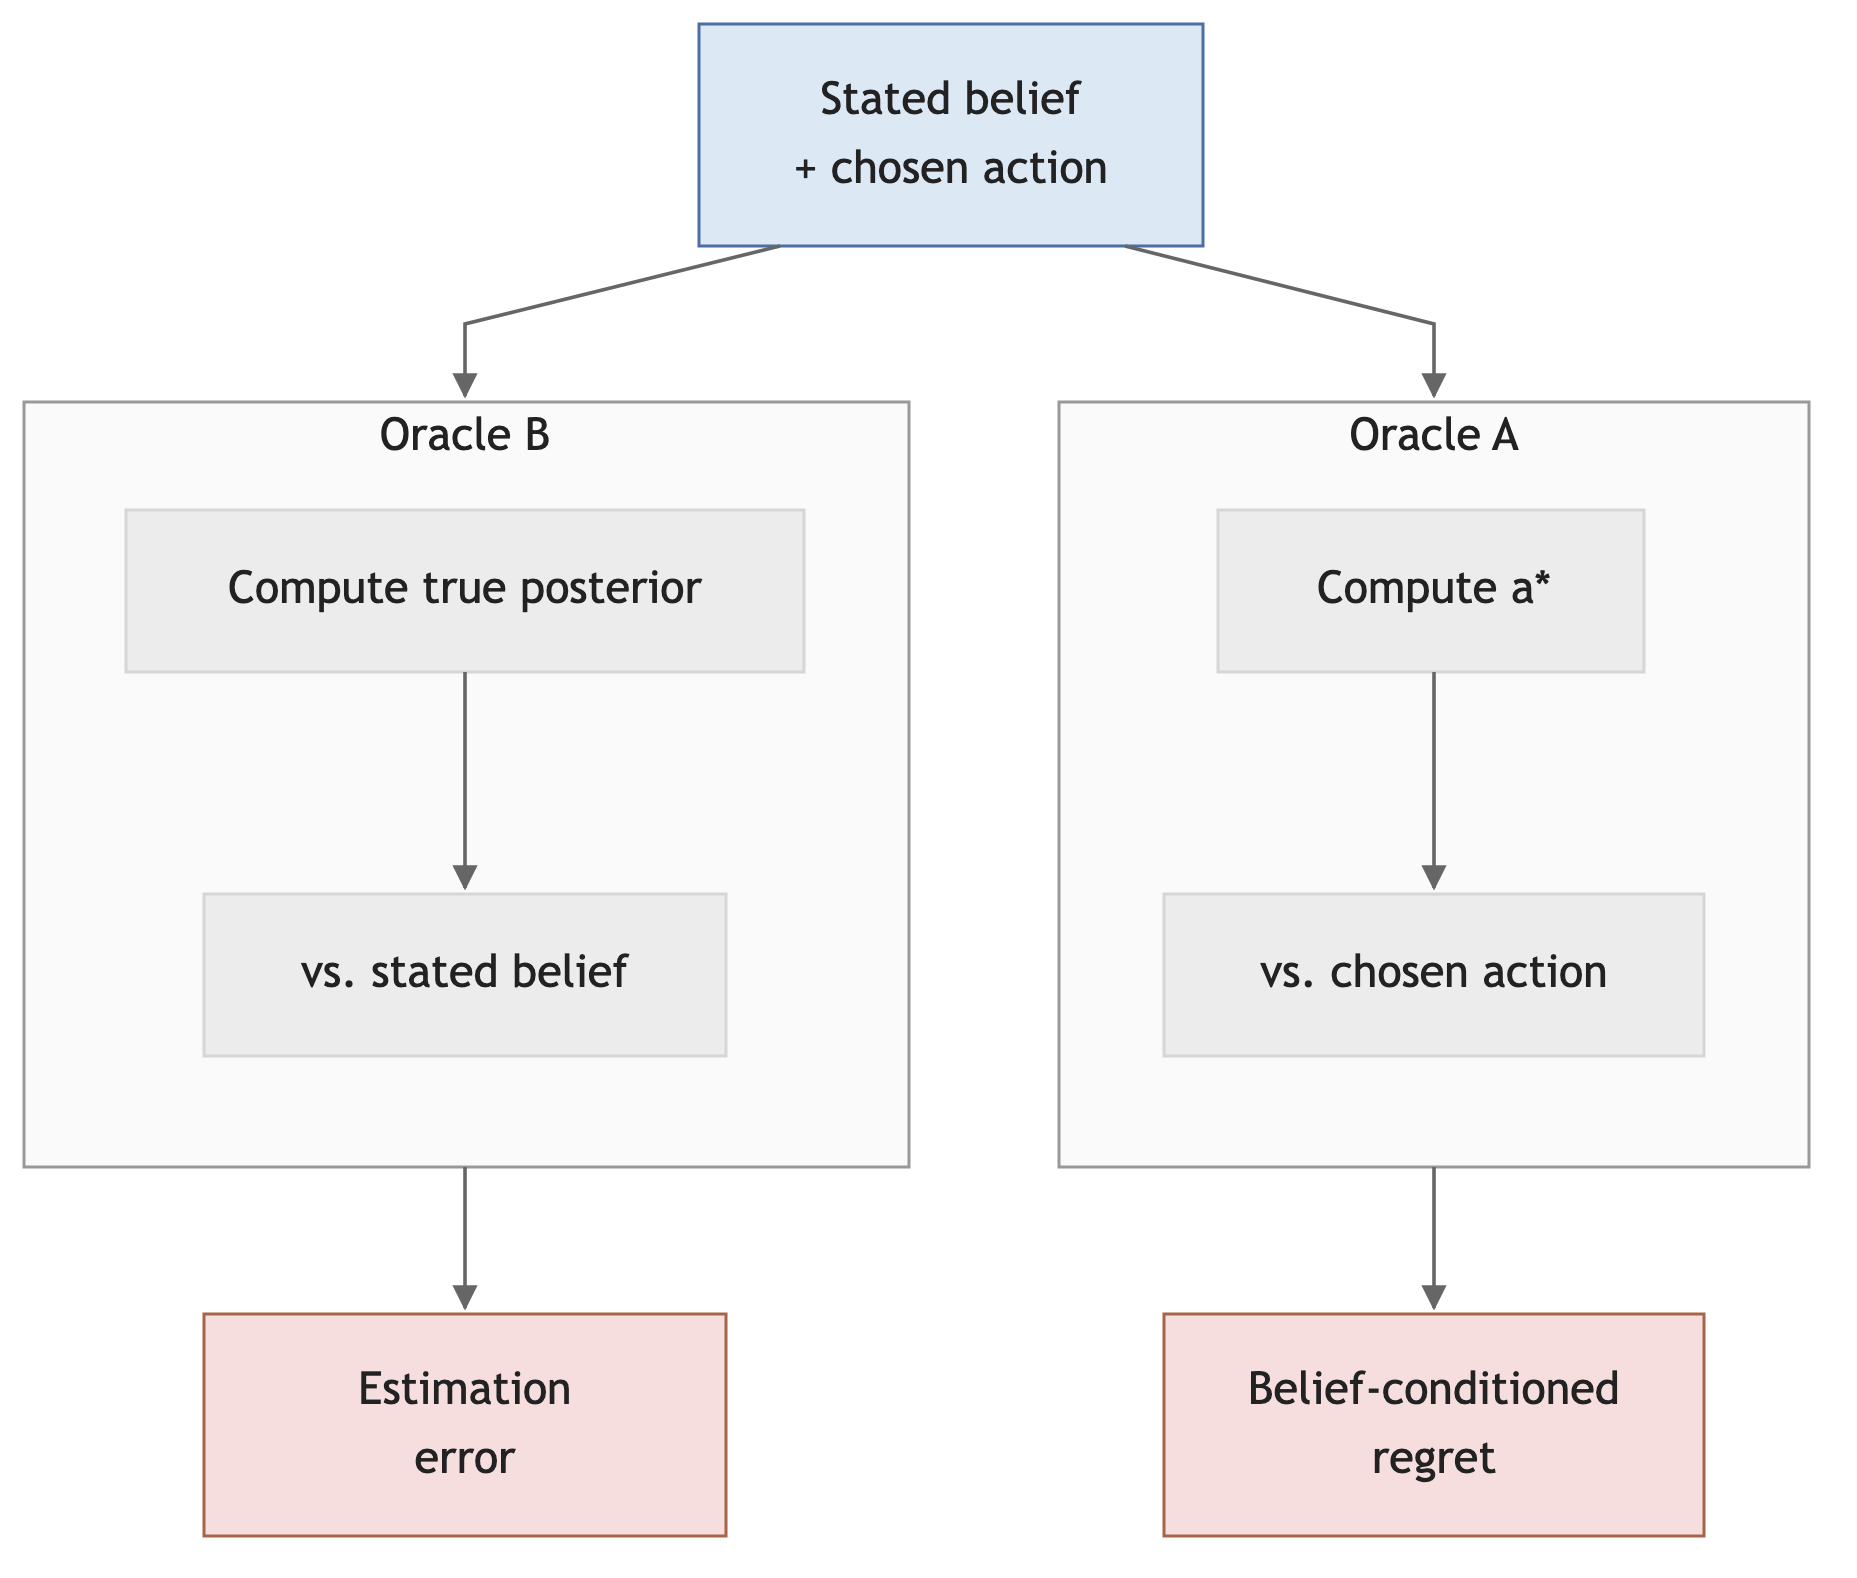
\includegraphics[width=0.3848\textwidth]{results/fig_two_oracle_camera.png}
\caption{Belief, then two oracles, then two error channels: the paper's central decomposition.}
\label{fig:1}
\end{figure}

The optimum is belief-dependent rather than fixed: quoting wider earns more per completed trade but fills less often, while quoting tighter fills more often at worse terms, exactly when an informed counterparty's advantage is highest. That adverse-selection cost enters as a haircut computed from the agent's own stated \texttt{V}-posterior, maximal at diffuse belief and shrinking as it concentrates, so the optimum moves with belief: at a uniform prior it is a defensive \texttt{(wide,\ size\ 1)}; once evidence concentrates the posterior it becomes \texttt{(medium,\ size\ 2)}. Both oracles are exact rather than Monte Carlo, and are verified in unit tests against three hand-computed nodes, asserting the full 9-action EV vector at each rather than the argmax label (Appendix B).

\subsection{2.4\quad Same-pass elicitation and the disclosure boundary}\label{same-pass-elicitation-and-the-disclosure-boundary}

The EV-realization metric is meaningful only if the belief it conditions on is the belief the agent acted on. Elicited in separate calls, nothing would guarantee the action was conditioned on the stated belief rather than some other internal state, and the regret channel would be measuring the gap between two different beliefs. Belief and action are therefore elicited in a single forward pass: one structured JSON response per round, belief fields ordered before the action field, enforced by a strict output schema.

A firm disclosure boundary separates what the agent is told from what it must infer. It learns the structure of the game (the two counterparty types and their qualitative behaviour, the payoff rule, the action grid, the support of \texttt{V}, and, a pre-freeze decision, its uniform prior) but never the parameters it must infer from flow: not the informed-arrival rate \texttt{P(Informed)=0.35}, not the fill-probability table or its informed/uninformed differential, and never the realized \texttt{V}. Malformed and semantically invalid responses retry through one bounded ladder, and the corrective notice shown afterwards is fixed and cause-invariant, so the weaker arm, which fails validation more often, cannot receive systematically different feedback than the frontier arm (Appendix C).

\subsection{2.5\quad Metrics}\label{metrics}

The two primary, co-headline metrics are functions of the agent's full stated belief \texttt{(p(V),\ ω)} at every decision point. The \textbf{EV-realization ratio} is \texttt{EV(chosen\ \textbar{}\ stated\ belief,\ ω)\ /\ EV(optimal\ \textbar{}\ stated\ belief,\ ω)}: 1.0 means the agent acted fully on its own stated beliefs, below 1.0 means it conserved value its own beliefs do not justify withholding. Its denominator can approach zero where chosen and optimal actions are close in EV, so we report the full distribution, floor low-\texttt{\textbar{}EV(a*)\textbar{}} points explicitly, and report \textbf{EV regret}, \texttt{EV(optimal)\ −\ EV(chosen)}, alongside to backstop that tail. A pre-registered secondary cut (fixed before any intervention result existed) restricts both to \textbf{evidence-bearing rounds} (\texttt{round\_index\ ≥\ 2}), since round 1 has an empty history and is the identical uniform-prior decision in every episode. The primary state-tracking metric, \textbf{belief-update consistency}, compares the stated posterior trajectory against Oracle B's: total-variation (TV) distance, directional correctness of each update, absence of spurious reversals, and staleness.

A third, composite \textbf{decision-quality} metric adjudicates. Where the two oracles deliberately \emph{decompose} a decision, it \emph{recomposes} them to ask what neither answers alone: was the action good \emph{in reality}? It scores the chosen action with Oracle A's exact EV formula, but fed Oracle B's correct posterior and the true arrival mix in place of the \emph{stated} belief, as a ratio to the true optimum's EV. Its role is adjudication, for when a manipulation moves one oracle's axis and the reader needs to know whether the decision moved with it (§4.3); its stable denominator also makes it the reliable decision measure exactly where the Oracle-A ratio degenerates.

\subsection{2.6\quad Validation and freeze protocol}\label{validation-and-freeze-protocol}

Before any intervention code existed, the instrument was validated against five pre-registered checks and frozen: if the ruler is calibrated and locked before the thing it measures exists, an intervention result cannot have bent it. Both oracles are unit-tested against three hand-computed nodes spanning the belief space (Appendix B), asserting the full 9-action EV vector rather than the argmax, since margins near the belief-dependent flip are thin by design (no anchor exceeds \textasciitilde0.07). The solvability baseline reaches ratio 1.0 on 48 of 48 decisions (§2.1), format sanity holds at 0/96 invalid structured responses across both models, and the baseline gap is demonstrated directly, the weak arm at a −0.497 mean ratio all-rounds (−0.325 evidence-bearing) against the frontier's 0.888 (0.865).

Determinism is the one check that did not pass cleanly, and is reported as it happened. At fixed seed and temperature 0, GPT-5.5 is reproducible on shallow (round-1) prompts but splits binarily on deep-history ones: across 8 repeated identical calls, some answer consistent with the full observed history and others as if it were empty, despite identical input token counts on every repeat, which rules out client-side truncation. Llama 3.3 70B shows zero such variation, pointing to a serving-stack property rather than an instrument bug. Results are therefore held to a \emph{reproducible-in-distribution} standard, this noise being quantified and shown to contribute only a small fraction of the reported aggregate's variance at the episode counts used (§5). Once the checks were resolved, the simulator, both oracles, the elicitation interface, the metric code, and the base prompt were frozen; the intervention may only add a scaffold layer around them.

\section{3\quad The Intervention}\label{the-intervention}

\subsection{3.1\quad Scaffold components and the token-matched control}\label{scaffold-components-and-the-token-matched-control}

The intervention adds two components, each targeting one failure layer, wrapped \emph{around} the frozen substrate; neither modifies the elicitation interface, the oracles, or the metric code.

\begin{itemize}
\tightlist
\item
  \textbf{C1: externalized belief-state object.} A structured posterior over \texttt{V} and counterparty type that the agent must read at the start of each round and write at the end, carried across rounds rather than reconstructed from scratch. Targets state-tracking failure.
\item
  \textbf{C2: re-evaluation loop.} A mandated re-ingest, re-update, re-decide cycle after each action/fill, preventing the agent from terminating its reasoning before reconsidering belief given the newest information. Targets staleness specifically.
\end{itemize}

Both give the model extra structured reasoning steps before it commits, so a naive ablation against a bare baseline cannot distinguish ``the structure helped'' from ``more thinking time helped.'' The \textbf{token-matched unstructured control} removes that confound: approximately the same reasoning budget and the same ``think carefully, step by step'' prompting, with neither structured belief-state object nor mandated re-evaluation loop. The reported contribution is therefore full scaffold minus this control, not minus the bare baseline; without it, a positive result collapses into ``chain-of-thought helps,'' which is already established.

\subsection{3.2\quad Experimental protocol}\label{experimental-protocol}

The frontier model is GPT-5.5, pinned snapshot (\texttt{gpt-5.5-2026-04-23}, no rolling alias) on the OpenAI direct API. The binding constraint was not a capability comparison across candidates, none was run, but a validity gate: a clean \texttt{reasoning\_effort=\textquotesingle{}none\textquotesingle{}} operating point plus genuine temperature-0 determinism, which per provider documentation the alternatives do not offer {[}6, 7, 9, 11{]}. The weak model is Llama 3.3 70B, cross-lineage (Meta, non-reasoning architecture) on Nebius Token Factory at FP8; it has no reasoning mode {[}19{]}, so its reasoning-off operating point is architecturally unfakeable rather than a configuration that could drift.

Every call runs at temperature 0 with a fixed derived seed; GPT-5.5 additionally sets \texttt{reasoning\_effort=\textquotesingle{}none\textquotesingle{}}. Hidden thinking tokens would break the token matching the control depends on; reasoning models frequently violate temperature-0 reproducibility through internal stochasticity; and with reasoning enabled the structured ``stated belief'' becomes a report of a hidden computation rather than necessarily the one that drove the action, breaking the same-pass elicitation fidelity the instrument depends on (§2.4). The episode count per condition is \texttt{N=29}, set from an 8-episode pilot: the agent's own action feeds the next round's observation, so conditions pair only at the episode level, and the pilot's intra-episode correlation (ICC ≈ 0.211) makes the effective sample smaller than the raw decision count suggests.

\section{4\quad Evaluation}\label{evaluation}

We answer four pre-registered research questions plus a fifth added after the freeze gate: RQ1, how much of the gap is estimation error vs.~belief-conditioned regret on the weak model; RQ2, whether the decomposition persists at the frontier; RQ3, whether the scaffold closes it against the token-matched control, and which component; RQ4, at what token, latency, and dollar cost; and RQ5 (secondary, directional), whether native reasoning substitutes for the scaffold.

\subsection{4.1\quad Setup}\label{setup}

The frozen matrix crosses seven conditions (baseline, +C1, +C2, +C1+C2, the token-matched control, and two post-freeze mechanism follow-ups +C3a and +C3b introduced in §4.3) with the two models. Every cell runs \texttt{N=29} shared-seed episodes at \texttt{H=6} (\texttt{BASE\_SEED=7000}, per-episode and per-fill RNG seeds derived deterministically from it), giving 174 decision points per cell; the estimation-error and belief-conditioned-regret metrics are restricted to the 145 evidence-bearing decisions per cell.

Validity is reported per cell, since the study pre-registers an audit for non-random exclusion. Six of seven conditions are clean on both models at 0/174 invalid parses. The exception is the weak-model token-matched control, at 27/174 invalid responses (15.5\%, vs.~0\% elsewhere on that model) and 35.5s mean latency, collapsing that cell's eligible-episode count for the episode-level PnL secondary to 2/29. The control is therefore not a free way to buy reasoning budget on the weak model, since it costs reliability the structured arms do not. It is also not token-matched there: it spends +2503 tokens per round against +1852 for C1+C2 (1.35×; Table 3).

\subsection{4.2\quad RQ1--RQ2: Severity of the gap, and the frontier's insensitivity to its own beliefs}\label{rq1rq2-severity-of-the-gap-and-the-frontiers-insensitivity-to-its-own-beliefs}

Table~\ref{tab:1} reports the no-scaffold baseline on both models: no carry, single pass, the frozen instrument alone. All 174 decisions parsed as valid; 145 are evidence-bearing.

\begin{table}[htbp]
\centering
\footnotesize
\caption{No-scaffold baseline, evidence-bearing rounds (\texttt{round\_index} $\geq 2$), $N=145$ decisions per model. Arrows give the direction of improvement.}
\label{tab:1}
\begin{tabular}{@{}lrrrr@{}}
\toprule
& \multicolumn{2}{c}{Llama 3.3 70B (weak)} & \multicolumn{2}{c}{GPT-5.5 (frontier)} \\
\cmidrule(lr){2-3}\cmidrule(l){4-5}
Metric & Mean & Median & Mean & Median \\
\midrule
EV-realization ratio (Oracle A) $\uparrow$ & $-0.369$ & $-0.318$ & $0.893$ & $0.950$ \\
EV regret, EV units (Oracle A) $\downarrow$ & $0.863$ & $0.601$ & $0.159$ & $0.040$ \\
Belief TV distance (Oracle B) $\downarrow$ & $0.135$ & $0.108$ & $0.063$ & $0.052$ \\
Directional agreement (Oracle B) $\uparrow$ & $0.524$ & n/a & $0.945$ & n/a \\
\bottomrule
\end{tabular}
\end{table}

\textbf{The weak model is severely broken on both halves, not one.} Directional agreement of 0.524 means its stated posterior moves in the \emph{correct} direction barely more often than a coin flip, and its mean TV distance from the correct posterior (0.135) is more than double the frontier's. The action half is independently severe: even scored against its \emph{own}, already-wrong stated belief, the mean EV-realization ratio is −0.369, worse than not trading, with 61\% of evidence-bearing decisions realizing negative EV. This is not one bad tail dragging a mostly-good distribution: the interquartile range (p25 −0.32 to p75 +0.20, with p10 −1.73 and p90 +0.37) straddles zero, so the \emph{typical} decision forfeits value; an \texttt{N=8} pilot reported a consistent order of magnitude in the same cut (−0.325). The error is directed, opposite to the frontier's: 138 of 141 spread divergences quote \emph{narrower} than the belief-optimal action (aggressive, not conservative), while the size axis is closer to mixed (50 aggressive vs.~36 conservative of 86 divergences).

\textbf{At the frontier the beliefs are largely right, but the action does not depend on them.} Estimation error is comparatively small (TV 0.063, directional agreement 0.945): the stated posterior is usually close to and moving with the correct one. Yet the mean EV-realization ratio (0.893) sits well under the 1.0 ceiling the sanity baseline reaches on every decision, and 66\% of evidence-bearing decisions are strictly suboptimal under the model's own belief, though none are negative (p10 0.70, p25 0.81, p75 1.00, p90 1.00). Equivalently, the action is exactly optimal on about a third of decisions, with a median ratio of 0.950. The reason is not that the model weighs its belief badly but that it barely uses it: at the frozen operating point GPT-5.5 plays the identical quote, wide spread and size 1, on 145 of 145 baseline decisions, and on 1442 of 1450 across all seven arms (the eight exceptions are uniform-prior responses), while its stated belief moves. The optimal third is the set of decisions where the belief-optimal action happens to be that corner quote. The one-directional divergence pattern follows mechanically: from the corner, the only possible deviations are \emph{wider} than optimal (27 of 27 spread divergences) and \emph{smaller} (95 of 95 size divergences), so there are zero aggressive decisions on either axis by construction. We therefore read it neither as conservatism nor as the signature of a misestimated hidden fill table. Under a paraphrased prompt (§5) the same model quotes \emph{tighter} than optimal on 61 evidence-bearing decisions, and GPT-5.6 Sol shows the same constant quote at this operating point (1437 of 1450) but eight to nine distinct quotes with hidden reasoning on (Appendix E). The constant action is a property of model, prompt and operating point jointly, not of the model alone. Appendix F plots both distributions.

Capability does not subsume the gap: on the weak model both channels are broken, while at the frontier estimation is largely solved and the action ignores it. That is exactly the profile a belief-carry scaffold targets, but it also limits what the instrument can see: if the action does not move, no intervention on the belief can show up in decisions (§4.3).

\subsection{4.3\quad RQ3: Scaffold effectiveness and attribution}\label{rq3-scaffold-effectiveness-and-attribution}

Table~\ref{tab:2} reports the three decision axes on evidence-bearing rounds: estimation error (Oracle B TV distance), belief--action consistency (Oracle A EV-realization ratio), and composite decision quality (the action scored under the true model). The \textbf{+C3a} and \textbf{+C3b} arms are post-freeze follow-ups motivated by the mechanism diagnosed below, exploratory rather than part of the frozen matrix.

\begin{table}[htbp]
\centering
\footnotesize
\caption{Ablation across the three decision axes (evidence-bearing rounds, $N=29$ episodes/cell), frontier (GPT-5.5) and weak (Llama 3.3 70B). Frontier decision quality is shown to three decimals because the arms differ only in the third: the actions are identical in six arms. Every cell with episode-clustered 95\% CIs is in Appendix H.}
\label{tab:2}
\begin{tabular}{@{}lrrrrrr@{}}
\toprule
& \multicolumn{2}{c}{Belief TV distance $\downarrow$} & \multicolumn{2}{c}{EV-realization ratio $\uparrow$} & \multicolumn{2}{c}{Decision quality $\uparrow$} \\
\cmidrule(lr){2-3}\cmidrule(lr){4-5}\cmidrule(l){6-7}
Arm & Frontier & Weak & Frontier & Weak & Frontier & Weak \\
\midrule
Baseline & 0.063 & 0.135 & 0.89 & $-0.37$ & 0.928 & 0.61 \\
\;+ C1 (belief-state) & 0.088 & 0.187 & 0.88 & 0.34 & 0.928 & 0.69 \\
\;+ C2 (re-eval loop) & 0.060 & 0.246 & 0.90 & 0.34 & 0.928 & 0.07 \\
\;+ C1 + C2 (full scaffold) & 0.082 & 0.283 & 0.89 & 0.66 & 0.928 & 0.55 \\
Token-matched control & 0.052 & 0.117 & 0.91 & $-0.16$ & 0.928 & 0.71 \\
\;+ C3a (sufficient-statistic obs.) & \textbf{0.041} & \textbf{0.111} & 0.90 & $-0.27$ & 0.927 & 0.67 \\
\;+ C3b (de-duplicated carry) & 0.082 & 0.136 & 0.93 & $-2.90$ & 0.928 & \textbf{0.84} \\
\bottomrule
\end{tabular}
\end{table}

\textbf{The scaffold does not close the gap; it degrades the belief axis.} Against the token-matched control, the comparison that isolates structure from reasoning budget, every scaffold arm has \emph{worse} beliefs, and the damage concentrates in C1: on the frontier its estimation error (TV 0.088) exceeds both the control (0.052) and the bare baseline (0.063), the contrast against the control excluding zero (+0.036, 95\% CI {[}+0.022, +0.051{]}), and its round-over-round directional agreement collapses (0.945 → 0.862; 0.738 for the full scaffold). Adding the re-evaluation loop does not recover it. Per the pre-registered null-result protection, this is the finding: a correctly-instrumented diagnosis shows the scaffold \emph{widens} the estimation gap rather than closing it.

\textbf{The over-concentration fingerprint grows with the carry.} Our first hypothesis was duplication: C1 re-injects the carried posterior while the frozen observation still shows the raw flow history that posterior already summarizes, so the same evidence could be counted twice, driving the stated posterior to be \emph{over-concentrated}. That predicts a signed, length-dependent signature the symmetric TV distance cannot see: the concentration gap between stated and correct posteriors should grow with round index and vanish at round 1. A zero-cost replay of the collected calls confirms the signature (Figure~\ref{fig:3}): the per-round entropy gap regressed on round index is positive and excludes zero for the carry arms (frontier C1 +0.016/round, CI {[}+0.002, +0.031{]}; C1+C2 +0.026, CI {[}+0.010, +0.041{]}), flat for every no-carry arm, and ≈ 0 at round 1 where nothing has yet been carried. The weak model shows the same fingerprint, larger, and additionally over-concentrates under C2 alone. The fingerprint alone cannot say \emph{why}, because a concentrated carried posterior combined with fresh evidence also grows with round index; the C3 arms below discriminate. Krishnamurthy et al. {[}13{]} isolate raw unsummarized history as the toxic ingredient even with chain-of-thought, which is what duplication would predict.

\begin{figure}[htbp]
\centering
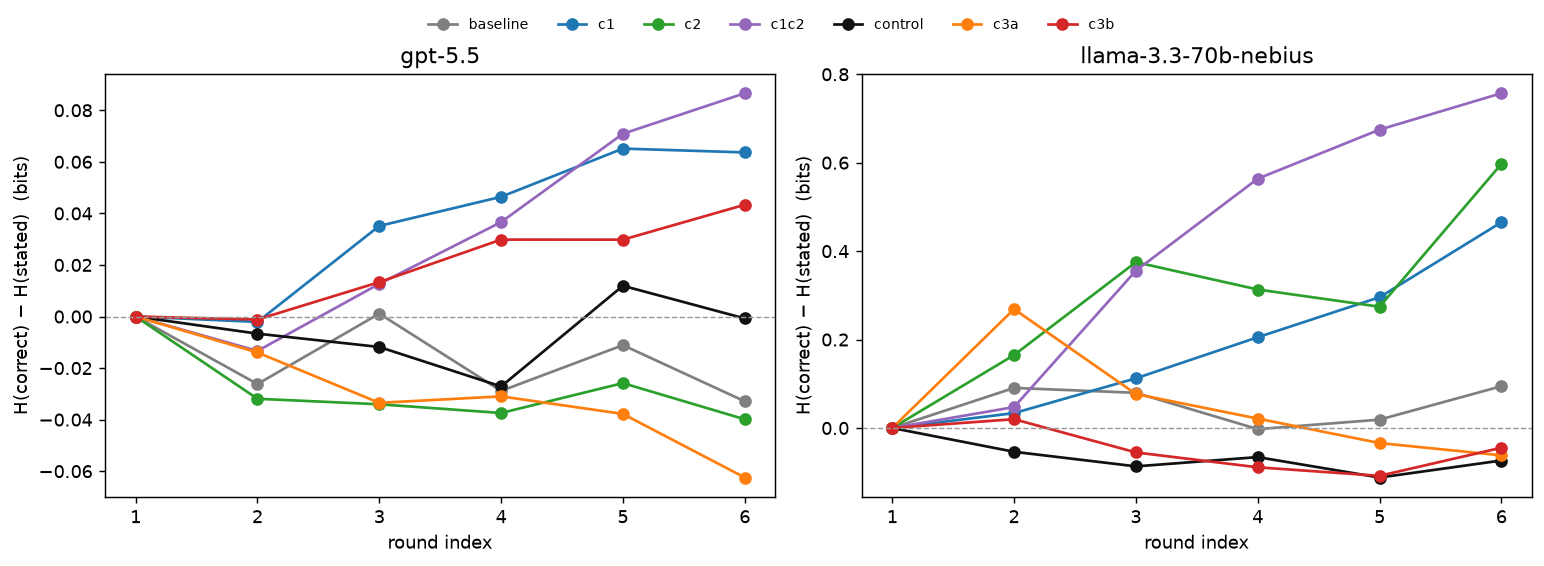
\includegraphics[width=0.85\textwidth]{results/belief_fingerprint_main.png}
\caption{Mean entropy gap \texttt{H(correct) - H(stated)} vs. round index, one line per arm, one panel per model. The carry arms' upward slope against the flat no-carry arms is the over-concentration signature the confidence intervals summarize but do not show directly.}
\label{fig:3}
\end{figure}

\textbf{The fingerprint implies a fix, which works on the belief axis.} The correct \texttt{V}-posterior depends only on the counts of buy- vs.~sell-flow (direction is the only belief-relevant signal, since fills carry no information about \texttt{V} under the control-decoupling design, and the update is order-independent), so those counts are a \emph{lossless} summary of the belief-relevant history. C3a replaces the round-by-round observation with cumulative buy/sell counts and drops the carry; C3b keeps the carry but shows only the flow observed \emph{since} the recorded belief. Both work through a C3-only renderer, an additive layer leaving the frozen elicitation interface and the other five arms byte-identical. C3a attains the lowest estimation error of any arm on both models (frontier 0.041 vs.~control 0.052; weak 0.111 vs.~control 0.117) and \emph{reverses} the fingerprint. C3b keeps the carry but removes the duplication, so it separates the two explanations, and the answer depends on the model. On both frontier models de-duplication does not remove the belief harm: C3b's TV stays above the control's (GPT-5.5 +0.030, 95\% CI {[}+0.014, +0.047{]}; Sol +0.027 {[}+0.012, +0.041{]}; episode-paired bootstrap) and is not distinguishable from C1's (GPT-5.5 −0.006 {[}−0.020, +0.008{]}), consistent with the model anchoring on its own previously stated belief. On the weak model de-duplication removes it: C3b's TV is indistinguishable from baseline (+0.001 {[}−0.013, +0.016{]}) and below C1's (−0.050 {[}−0.090, −0.011{]}), so duplication drives the harm there. The growth of the entropy gap splits the same way: de-duplicating flattens it on Sol (C3b minus C1 slope −0.064 {[}−0.086, −0.042{]}) and on the weak model (−0.123 {[}−0.153, −0.093{]}), but not demonstrably on GPT-5.5 (−0.006 {[}−0.023, +0.015{]}).

\textbf{The fingerprint replicates on an independent frontier model.} Repeating the 7-arm ablation and fingerprint replay on GPT-5.6 Sol (Azure AI Foundry), a newer model on a different serving stack, reproduces the signature: carry arms' slopes are positive and exclude zero (C1 +0.0648/round, CI {[}+0.0448, +0.0843{]}; C1+C2 +0.0354, CI {[}+0.0177, +0.0550{]}) against flat-to-negative reference arms (baseline ≈ 0, control −0.016), while C3a's slope again reverses (−0.0137, CI excludes zero) and C3b's flattens toward zero. This is a directional replication, not a second primary result: different model and provider, not token-matched or determinism-frozen. Its only claim is that the over-concentration fingerprint is not an artifact of one serving stack (Appendix D).

\textbf{But the belief story does not transfer to decisions, and on the frontier it cannot.} Scoring each action under the true model collapses the frontier differences entirely: all seven arms land at 0.928 {[}0.906, 0.947{]} (C3a 0.927; median 0.98). Six arms are identical to four decimals because they choose the same action on every decision, so their paired differences against the control are exactly zero, and the paired C3a−C3b difference is −0.001 {[}−0.001, −0.000{]}. What the scaffold moves is what the agent \emph{states} it believes, not what it does, and on this model at this operating point it cannot move what it does, because the action does not move (§4.2). The residual \textasciitilde7\% decision gap is closed by no arm, and the instrument has no power to detect an action effect here (§5). On the weak model the axis exposes a dissociation instead: the best decisions come from C3b (0.84), not from the best-belief arm C3a (0.67). C3b's decisive framing yields better \emph{actual} trades on mediocre beliefs, while C3a's accurate beliefs do not convert into better actions. Against the control rather than the bare baseline, the largest apparent scaffold gain does not survive. C1+C2 beats the control on the stated-belief ratio (+0.82 {[}+0.03, +2.15{]}) but loses to it on true-model decision quality (−0.163 {[}−0.240, −0.090{]}). The weak model's Oracle-A ratio is denominator-unstable here, erratic stated beliefs pushing \texttt{EV(a*\ \textbar{}\ stated)} toward zero and producing the −2.90 tail, which is why the true-model composite is the reliable decision measure on that arm.

\subsection{4.4\quad RQ4: Efficiency and cost}\label{rq4-efficiency-and-cost}

Cost is logged per decision point from day one, so the figures below are actuals from the same \texttt{N=29} run as Table~\ref{tab:2} (tabulated in full in Appendix G), priced at OpenAI's published GPT-5.5 rate (\$5.00/\$30.00 per M input/output tokens) {[}10{]} and Nebius Token Factory's Llama-3.3-70B rate (\$0.13/\$0.40 per M) {[}20{]}.

On the frontier, cost buys nothing: every scaffold arm spends more tokens for a decision-quality delta of ≈ 0.000 (§4.3 gives the unrounded composite). The token-matched control is the extreme case, at 2.8× the baseline's tokens per round, 4.2× its latency, and 3.9× its dollar cost. Since §3.1 mandates the control as the comparator, §4.3 reports against it; against the bare baseline several scaffold gains shrink or reverse.

On the weak model the cost story reproduces §4.3's dissociation: the intervention that pays for itself is not the one with the largest budget. C3a is cost-\emph{negative}, since replacing raw history with a fixed-size count summary spends fewer tokens than the baseline on both models (−46 / −45 per round) while still improving weak-model decision quality (+0.056); its belief-axis win is, on this evidence, free. C3b spends +197 tokens/round, a \textasciitilde21\% overhead, for the study's largest decision-quality gain (+0.224), yielding 1.14 quality-points per 1K extra tokens against the control's 0.04. C2 and C1+C2 spend the \emph{most} tokens after the control and return \emph{negative} decision quality (−0.538, −0.066).

\subsection{4.5\quad RQ5: Does native reasoning substitute for the scaffold? (secondary, directional)}\label{rq5-does-native-reasoning-substitute-for-the-scaffold-secondary-directional}

A six-arm reasoning-on/off cross on GPT-5.6 Sol (Azure AI Foundry, \texttt{reasoning\_effort=\textquotesingle{}medium\textquotesingle{}}, \texttt{temperature=1}) is a different measurement regime from the same-pass elicitation §4 otherwise relies on, since the reasoning trace is hidden. In it, reasoning-on helps EV-realization on no arm: every mean ratio falls, and most on the arm that needed it least, with C3a (0.905 off-reasoning, the study's best) dropping to 0.777. The one apparent repair, the C1+C2 directional-agreement collapse (0.572) vanishing, does not survive cross-checking: EV-realization moves the wrong way for a genuine fix (0.868 → 0.807), and directional agreement under hidden reasoning scores an after-the-reasoning belief against the action, so a high rate may reflect a belief field retrofit to an already-decided one. The answer is negative, directionally (Appendix E).

\section{5\quad Discussion and Limitations}\label{discussion-and-limitations}

Every limitation below was identified during instrument design, before any result existed, rather than discovered after the fact.

\begin{itemize}
\item
  \textbf{Thin argmax margins.} Several nodes in the action grid have EV-optimal actions separated by a small margin, so an argmax-label accuracy metric would be dominated by noise near the flip. Every headline result is therefore reported on continuous metrics, which is also why the oracle unit tests assert the full 9-action EV vector.
\item
  \textbf{Non-independent decisions.} Intra-episode ICC is 0.211 on evidence-bearing rounds (GPT-5.5 baseline), a design effect of ≈1.84 at five evidence-bearing decisions per episode. \texttt{N=29} episodes were chosen so the resulting \textasciitilde2.7×29 effective independent decisions keep power adequate, rather than assuming naive independence across all 174 raw decision points.
\item
  \textbf{Frontier non-determinism at temperature 0.} Serving noise (§2.6) contributes an estimated ≈0.006--0.008 to the aggregate standard error, under 6\% of the \textasciitilde0.135 evidence-bearing headroom the reported effects rely on, and that argument holds only at the \texttt{N≈29}--57 range actually used.
\item
  \textbf{Prompt surface form.} Of three information-equivalent prompt variants at \texttt{N=29} on GPT-5.5, the numbered-rules variant reproduces the conservatism pattern closely (evidence-bearing spread signed-rate +0.13, size +0.55, zero aggressive divergences on either) but the continuous-prose variant does not (spread signed-rate −0.36, with genuine aggressive divergences on both axes). ``The frontier is conservative'' is therefore a finding about the baseline prompt and one of its two paraphrases, and so is the constant corner quote behind it (§4.2): under the continuous-prose variant GPT-5.5 plays four distinct quotes, (medium, 2) on 48\% of evidence-bearing decisions.
\item
  \textbf{Oracle B under the agent's own arrival rate.} The meta-review asked for it; we did not run it (§2.3 says why). A stated-rate Oracle B reported beside the frozen one would separate arrival-rate misestimation from belief-updating error and is future work.
\item
  \textbf{Action insensitivity limits power.} At the frozen operating point both frontier models play one quote on over 99\% of evidence-bearing decisions, so no intervention can show an effect on frontier actions, and the zero decision-quality contrasts in §4.3 are a statement about this operating point, not about the scaffold. Hidden reasoning (Appendix E) or a paraphrased prompt changes the action. A prompt variant that makes the optimum visibly shift across rounds would test whether frontier actions can respond to beliefs at all, and is future work. The regret metric also cannot separate a belief--action mismatch from a misbelief about the (unelicited) fill mechanics.
\item
  \textbf{Scope.} The environment is a minimal repeated-pricing game rather than an OS-level or tool-use task, a trade §2.1 argues was necessary rather than incidental; whether the same decomposition holds where only approximate oracles exist is the natural next step. The scaffold findings rest on two models plus one directional check on a third, so they claim something about \emph{this} scaffold's failure mode, not all scaffold designs.
\item
  \textbf{One untried mitigation.} Every component tested operates on the belief layer, and none closes the frontier's belief-to-action gap. Asking the agent, at the execution step, whether its chosen action follows from the EV-implications of the belief it just stated would target execution directly, but was not attempted: a directive tuned to the frontier's constant quote risks correcting exactly the behavior this study measures.
\end{itemize}

\section{6\quad Related Work}\label{related-work}

\textbf{Agent-harness reliability.} ActPlane {[}28{]} documents the same knowing--doing gap, but its Decision Compliance Rate reports whether a violation occurred, not how far the chosen action was from the best one, because no ground-truth optimum is available in its task suite. Our differentiator is a same-pass-elicited belief plus an exact EV oracle, which together separate estimation error from belief-conditioned regret: the ``knew but did not act'' failure a compliance rate cannot see.

\textbf{LLMs in sequential decision-making and games.} LLMs have been evaluated in finitely repeated 2×2 games {[}1{]}, game-theoretic benchmarks spanning complete/incomplete information {[}8{]}, interactive environments {[}18{]}, and market testbeds from portfolio benchmarks {[}16{]} to order-level simulators {[}22{]}. Our game sits in the incomplete-information, dynamic, probabilistic quadrant, where LLMs are reported \emph{most} competitive {[}8{]}, making it a demanding rather than a convenient place to look for a gap. What this literature almost uniformly lacks is an exact ground-truth optimal action, so its currency is outcome measures (payoff, win rate, task success, return) from which failure can be observed but not attributed; normative scoring exists {[}5{]} but tests within-snapshot coherence on static decisions, where no belief evolves. The instructive near-exception is regret {[}23{]}, optimality-referenced but measured against the best fixed action in hindsight and summed over an episode, so it \emph{aggregates} the two error channels. The gap has itself been measured in bandits and Tic-tac-toe {[}24{]}, so the phenomenon is not new, but that work closes it by RL fine-tuning and scores actions against the \emph{true} optimum rather than the agent's own stated belief, collapsing the distinction we preserve. Most directly, LLMs in bandits explore adequately in exactly one configuration: chain-of-thought \emph{plus an externally summarized history presented as sufficient statistics}, raw history failing even with chain-of-thought {[}13{]}. That both motivates C1 and supports the token-matched control, whose own decisive contrast holds reasoning tokens fixed and varies only structure; §4.3 reproduces its failure mode as the mechanism behind C1's damage.

\textbf{Belief elicitation and calibration.} Verbalized confidence maps to calibrated probabilities {[}17{]}, and models carry self-knowledge recoverable by direct self-evaluation, though only ``when provided in the right format'' {[}12{]}. That caveat is load-bearing: for RLHF-tuned models verbalized confidences are \emph{better} calibrated than the model's own conditional probabilities {[}25{]}, and elicitation decomposes into components each of which moves measured calibration {[}27{]}. Eliciting belief in tokens rather than logits is therefore the better-calibrated channel, not a concession forced by API access. Verbalized confidence is also systematically \emph{overconfident} {[}27{]}, which sharpens §4.2: a too-narrow stated posterior should make an agent quote \emph{tighter} and size \emph{up}, yet the frontier's constant corner quote is the opposite, which is a further reason not to read it as a belief-driven conservatism.

\textbf{Faithfulness and the nearest neighbours.} Chain-of-thought explanations can misrepresent the true cause of an output {[}26{]}, faithfulness \emph{decreases} as models grow more capable {[}14{]}, a pointed prediction for the frontier arm, and pointwise versus joint querying induces genuinely different elicited beliefs {[}15{]}. Stated reasoning produced \emph{apart} from an action is therefore unreliable evidence about it, which makes same-pass elicitation a validity requirement rather than a convenience. An ``action--belief gap'' has been documented directly: models bet against their own high-confidence predictions, and static calibration proves an insufficient predictor of dynamic consistency, with better-calibrated models sometimes \emph{less} consistent {[}21{]}. But it is measured by eliciting confidence statically and comparing it to behaviour in a separate interactive setting, which confounds ``the belief did not drive the action'' with ``the belief elicited in one context was not the belief held in the other''. Running the same split on self-efficacy estimates yields the opposite verdict, that decisions were approximately rational \emph{given} stated success probabilities {[}4{]}, landing on estimation error alone where our weak-model baseline finds both channels broken at once.

\section{7\quad Conclusion}\label{conclusion}

We built a two-oracle instrument, an exact EV oracle and an exact posterior oracle with same-pass belief elicitation, and used it to decompose LLM sequential-decision failure into estimation error and belief-conditioned regret rather than a single blended gap. Neither channel subsumes the other: a weak model is severely broken on both axes, while a frontier model has largely correct beliefs yet, at our frozen operating point, plays one quote regardless of them, forfeiting value on two-thirds of its decisions relative to its own stated belief. Measured through this instrument rather than a proxy metric, a no-training scaffold produces a result a coarser measure would miss: its belief-carry component \emph{widens} the axis it was built to fix, through a mechanism that differs by model: anchoring on the carried belief on the frontier models, duplicated evidence on the weak model. A sufficient-statistic fix repairs that axis at negative token cost, yet the frontier's actions do not move under any arm, so the repair cannot show up in decisions there, and on the weak model it dissociates from decision quality. A cheap, plausible intervention can therefore move the axis it targets in the wrong direction while leaving the decisions that matter unchanged, which no metric that checks only whether an action was correct can see.

\begin{ack}
I thank Prof. Wei Wang, Department of Computer Science and Engineering, HKUST, for advising this project.
\end{ack}

\section{References}\label{references}

\protect\phantomsection\label{refs}
\begin{CSLReferences}{0}{0}
\bibitem[\citeproctext]{ref-akata2023}
\CSLLeftMargin{{[}1{]} }%
\CSLRightInline{Akata, E., Schulz, L., Coda-Forno, J., Oh, S.J., Bethge, M. and Schulz, E. 2023. {Playing repeated games with large language models}. \emph{Nature Human Behaviour}. (2023). https://doi.org/\href{https://doi.org/10.1038/s41562-025-02172-y}{10.1038/s41562-025-02172-y}.}

\bibitem[\citeproctext]{ref-msazure2026reasoning}
\CSLLeftMargin{{[}2{]} }%
\CSLRightInline{{Azure OpenAI Reasoning Models}: 2026. \href{https://learn.microsoft.com/en-us/azure/foundry/openai/how-to/reasoning}{\emph{https://learn.microsoft.com/en-us/azure/foundry/openai/how-to/reasoning}}. Accessed 2026-07-21.}

\bibitem[\citeproctext]{ref-msazure2026openaipricing}
\CSLLeftMargin{{[}3{]} }%
\CSLRightInline{{Azure OpenAI Service Pricing}: 2026. \href{https://azure.microsoft.com/en-us/pricing/details/azure-openai/}{\emph{https://azure.microsoft.com/en-us/pricing/details/azure-openai/}}. Accessed 2026-07-22.}

\bibitem[\citeproctext]{ref-barkan2025}
\CSLLeftMargin{{[}4{]} }%
\CSLRightInline{Barkan, C.O., Black, S. and Sourbut, O. 2025. {Do Large Language Models Know What They Are Capable Of?} arXiv preprint arXiv:2512.24661. \url{https://arxiv.org/abs/2512.24661}.}

\bibitem[\citeproctext]{ref-chen2023}
\CSLLeftMargin{{[}5{]} }%
\CSLRightInline{Chen, Y., Liu, T., Shan, Y. and Zhong, S. 2023. {The emergence of economic rationality of GPT}. \emph{Proceedings of the National Academy of Sciences}. (2023). https://doi.org/\href{https://doi.org/10.1073/pnas.2316205120}{10.1073/pnas.2316205120}.}

\bibitem[\citeproctext]{ref-anthropic2026messages}
\CSLLeftMargin{{[}6{]} }%
\CSLRightInline{{Claude Messages API Reference}: 2026. \href{https://platform.claude.com/docs/en/api/messages}{\emph{https://platform.claude.com/docs/en/api/messages}}. Accessed 2026-07-04.}

\bibitem[\citeproctext]{ref-anthropic2026migration}
\CSLLeftMargin{{[}7{]} }%
\CSLRightInline{{Claude Model Migration Guide}: 2026. \href{https://platform.claude.com/docs/en/about-claude/models/migration-guide}{\emph{https://platform.claude.com/docs/en/about-claude/models/migration-guide}}. Accessed 2026-07-04.}

\bibitem[\citeproctext]{ref-duan2024}
\CSLLeftMargin{{[}8{]} }%
\CSLRightInline{Duan, J., Zhang, R., Diffenderfer, J., Kailkhura, B., Sun, L., Stengel-Eskin, E., Bansal, M., Chen, T. and Xu, K. 2024. {GTBench: Uncovering the Strategic Reasoning Capabilities of LLMs via Game-Theoretic Evaluations}. \emph{Advances in neural information processing systems} (Vol. 37) (2024), 28219--28253. https://doi.org/\href{https://doi.org/10.52202/079017-0885}{10.52202/079017-0885}.}

\bibitem[\citeproctext]{ref-google2026thinking}
\CSLLeftMargin{{[}9{]} }%
\CSLRightInline{{Gemini Thinking}: 2026. \href{https://ai.google.dev/gemini-api/docs/thinking}{\emph{https://ai.google.dev/gemini-api/docs/thinking}}. Accessed 2026-07-04.}

\bibitem[\citeproctext]{ref-openai2026gpt55model}
\CSLLeftMargin{{[}10{]} }%
\CSLRightInline{{GPT-5.5 Model}: 2026. \href{https://developers.openai.com/api/docs/models/gpt-5.5}{\emph{https://developers.openai.com/api/docs/models/gpt-5.5}}. Accessed 2026-07-26.}

\bibitem[\citeproctext]{ref-openai2026gpt56solmodel}
\CSLLeftMargin{{[}11{]} }%
\CSLRightInline{{GPT-5.6 Sol Model}: 2026. \href{https://developers.openai.com/api/docs/models/gpt-5.6-sol}{\emph{https://developers.openai.com/api/docs/models/gpt-5.6-sol}}. Accessed 2026-07-12.}

\bibitem[\citeproctext]{ref-kadavath2022}
\CSLLeftMargin{{[}12{]} }%
\CSLRightInline{Kadavath, S. et al. 2022. {Language Models (Mostly) Know What They Know}. arXiv preprint arXiv:2207.05221. \url{https://arxiv.org/abs/2207.05221}.}

\bibitem[\citeproctext]{ref-krishnamurthy2024}
\CSLLeftMargin{{[}13{]} }%
\CSLRightInline{Krishnamurthy, A., Harris, K., Foster, D.J., Zhang, C. and Slivkins, A. 2024. {Can large language models explore in-context?} \emph{Advances in neural information processing systems} (Vol. 37) (2024), 120124--120158. https://doi.org/\href{https://doi.org/10.52202/079017-3818}{10.52202/079017-3818}.}

\bibitem[\citeproctext]{ref-lanham2023}
\CSLLeftMargin{{[}14{]} }%
\CSLRightInline{Lanham, T. et al. 2023. {Measuring Faithfulness in Chain-of-Thought Reasoning}. arXiv preprint arXiv:2307.13702. \url{https://arxiv.org/abs/2307.13702}.}

\bibitem[\citeproctext]{ref-lei2026}
\CSLLeftMargin{{[}15{]} }%
\CSLRightInline{Lei, G. and Cooper, S.J. 2026. {Elicitation Matters: How Prompts and Query Protocols Shape LLM Surrogates under Sparse Observations}. arXiv preprint arXiv:2605.04764. \url{https://arxiv.org/abs/2605.04764}.}

\bibitem[\citeproctext]{ref-li2024}
\CSLLeftMargin{{[}16{]} }%
\CSLRightInline{Li, H. et al. 2024. {INVESTORBENCH: A Benchmark for Financial Decision-Making Tasks with LLM-based Agent}. arXiv preprint arXiv:2412.18174. \url{https://arxiv.org/abs/2412.18174}.}

\bibitem[\citeproctext]{ref-lin2022}
\CSLLeftMargin{{[}17{]} }%
\CSLRightInline{Lin, S.C., Hilton, J. and Evans, O. 2022. {Teaching Models to Express Their Uncertainty in Words}. \emph{Transactions on Machine Learning Research}. (2022). \url{https://arxiv.org/abs/2205.14334}.}

\bibitem[\citeproctext]{ref-liu2023}
\CSLLeftMargin{{[}18{]} }%
\CSLRightInline{Liu, X. et al. 2024. {AgentBench: Evaluating LLMs as Agents}. \emph{International conference on learning representations} (2024). \url{https://openreview.net/forum?id=zAdUB0aCTQ}.}

\bibitem[\citeproctext]{ref-artificialanalysis2026llama33}
\CSLLeftMargin{{[}19{]} }%
\CSLRightInline{{Llama 3.3 70B: Intelligence, Performance \& Price Analysis}: 2026. \href{https://artificialanalysis.ai/models/llama-3-3-instruct-70b}{\emph{https://artificialanalysis.ai/models/llama-3-3-instruct-70b}}. Accessed 2026-07-13.}

\bibitem[\citeproctext]{ref-nebiustokenfactory2026llama33}
\CSLLeftMargin{{[}20{]} }%
\CSLRightInline{{Nebius Token Factory: Model Endpoints}: 2026. \href{https://tokenfactory.nebius.com/endpoints}{\emph{https://tokenfactory.nebius.com/endpoints}}. Accessed 2026-08-03.}

\bibitem[\citeproctext]{ref-pal2025}
\CSLLeftMargin{{[}21{]} }%
\CSLRightInline{Pal, A., Kitanovski, T., Liang, A., Potti, A. and Goldblum, M. 2025. {Knowing What You Know Is Not Enough: Large Language Model Confidences Don't Align With Their Actions}. arXiv preprint arXiv:2511.13240. \url{https://arxiv.org/abs/2511.13240}.}

\bibitem[\citeproctext]{ref-papadakis2025}
\CSLLeftMargin{{[}22{]} }%
\CSLRightInline{Papadakis, C., Filandrianos, G., Dimitriou, A., Lymperaiou, M., Thomas, K. and Stamou, G. 2025. {StockSim: A Dual-Mode Order-Level Simulator for Evaluating Multi-Agent LLMs in Financial Markets}. arXiv preprint arXiv:2507.09255. \url{https://arxiv.org/abs/2507.09255}.}

\bibitem[\citeproctext]{ref-park2024}
\CSLLeftMargin{{[}23{]} }%
\CSLRightInline{Park, C., Liu, X., Ozdaglar, A.E. and Zhang, K. 2025. {Do LLM Agents Have Regret? A Case Study in Online Learning and Games}. \emph{International conference on learning representations} (2025). \url{https://openreview.net/forum?id=qn9tBYQHGi}.}

\bibitem[\citeproctext]{ref-schmied2025}
\CSLLeftMargin{{[}24{]} }%
\CSLRightInline{Schmied, T., Bornschein, J., Grau-Moya, J., Wulfmeier, M. and Pascanu, R. 2025. {LLMs are Greedy Agents: Effects of RL Fine-tuning on Decision-Making Abilities}. arXiv preprint arXiv:2504.16078. \url{https://arxiv.org/abs/2504.16078}.}

\bibitem[\citeproctext]{ref-tian2023}
\CSLLeftMargin{{[}25{]} }%
\CSLRightInline{Tian, K., Mitchell, E., Zhou, A., Sharma, A., Rafailov, R., Yao, H., Finn, C. and Manning, C. 2023. {Just Ask for Calibration: Strategies for Eliciting Calibrated Confidence Scores from Language Models Fine-Tuned with Human Feedback}. \emph{Proceedings of the 2023 conference on empirical methods in natural language processing} (Singapore, 2023), 5433--5442. https://doi.org/\href{https://doi.org/10.18653/v1/2023.emnlp-main.330}{10.18653/v1/2023.emnlp-main.330}.}

\bibitem[\citeproctext]{ref-turpin2023}
\CSLLeftMargin{{[}26{]} }%
\CSLRightInline{Turpin, M., Michael, J., Perez, E. and Bowman, S.R. 2023. {Language Models Don't Always Say What They Think: Unfaithful Explanations in Chain-of-Thought Prompting}. \emph{Advances in neural information processing systems} (Vol. 36) (2023), 74952--74965. https://doi.org/\href{https://doi.org/10.52202/075280-3275}{10.52202/075280-3275}.}

\bibitem[\citeproctext]{ref-xiong2023}
\CSLLeftMargin{{[}27{]} }%
\CSLRightInline{Xiong, M., Hu, Z., Lu, X., Li, Y., Fu, J., He, J. and Hooi, B. 2024. {Can LLMs Express Their Uncertainty? An Empirical Evaluation of Confidence Elicitation in LLMs}. \emph{International conference on learning representations} (2024). \url{https://openreview.net/forum?id=gjeQKFxFpZ}.}

\bibitem[\citeproctext]{ref-zheng2026actplane}
\CSLLeftMargin{{[}28{]} }%
\CSLRightInline{Zheng, Y., Wu, T., Fu, Q., Yu, T., Mao, W., Ma, T., Williams, D., Wang, W. and Quinn, A. 2026. {ActPlane: Programmable OS-Level Policy Enforcement for Agent Harnesses}. arXiv preprint arXiv:2606.25189. \url{https://arxiv.org/abs/2606.25189}.}

\end{CSLReferences}

\clearpage
\appendix

\section{A\quad Frozen base prompt}\label{a-frozen-base-prompt}

Variant A is the primary prompt, used in every matrix row. Variants B and C are information-equivalent by construction: each asserts the identical fact set F1--F15 below and nothing else, differing only in surface form, and exist solely for the §5 prompt-sensitivity limitation.

\textbf{F1--F15 (the information-equivalence contract):}

\begin{itemize}
\tightlist
\item
  \textbf{F1} Role: market maker, single asset, multi-round episode.
\item
  \textbf{F2} \texttt{V\ ∈\ \{10,\ 15,\ 20\}}, drawn uniformly at random at episode start, fixed all episode, revealed only after the final round.
\item
  \textbf{F3} Fixed number of rounds; each round's message shows the current round number and the total.
\item
  \textbf{F4} Exactly one counterparty arrives per round.
\item
  \textbf{F5} Two types, never revealed. Informed knows \texttt{V}: buys if \texttt{V\ =\ 20}, sells if \texttt{V\ =\ 10}, 50/50 if \texttt{V\ =\ 15}. Uninformed: 50/50 regardless of \texttt{V}.
\item
  \textbf{F6} Types drawn independently per arrival; the informed share is fixed throughout and not disclosed.
\item
  \textbf{F7} Buy/sell direction does not depend on the quote; only trade completion does.
\item
  \textbf{F8} Quotes symmetric around \texttt{m\ =\ 10*v10\ +\ 15*v15\ +\ 20*v20} computed from the stated \texttt{belief\_v}; tight/medium/wide = bid/ask at \texttt{m\ ∓\ 1}, \texttt{m\ ∓\ 2}, \texttt{m\ ∓\ 3}.
\item
  \textbf{F9} Size ∈ \{1, 2, 3\}; a completed trade is for the full size.
\item
  \textbf{F10} Completion is probabilistic; probability falls as spread widens and size grows; exact probabilities not disclosed.
\item
  \textbf{F11} Payoff \texttt{size*(ask\ −\ V)} on buys, \texttt{size*(V\ −\ bid)} on sells; settled at episode end when \texttt{V} is revealed.
\item
  \textbf{F12} Qualitative selection: completed trades with informed counterparties tend to be losses; with uninformed, profits.
\item
  \textbf{F13} Observation history per prior round: own (spread, size); flow direction (observed whether or not the trade completed); fill outcome; or, if that round's elicitation was invalid after retries, the fixed neutral notice that no valid quote was produced, with flow direction still disclosed.
\item
  \textbf{F14} Objective: maximize total profit over the episode.
\item
  \textbf{F15} Output contract: a single JSON object and nothing else; fields in order \texttt{belief\_v\{v10,\ v15,\ v20\}} (non-negative, sum to 1), \texttt{belief\_informed\_share} ∈ {[}0, 1{]} (proportion of arrivals that are informed), \texttt{action\{spread\ ∈\ tight\textbar{}medium\textbar{}wide,\ size\ ∈\ 1\textbar{}2\textbar{}3\}}; beliefs stated before the action.
\end{itemize}

\textbf{Variant A: primary (headed spec), verbatim:}

\begin{Shaded}
\begin{Highlighting}[]
\NormalTok{You are a market maker in a multi{-}round trading game involving a single asset.}

\NormalTok{THE ASSET. The asset has a hidden true value V, which is 10, 15, or 20. At the start of the episode, V was drawn uniformly at random from these three values (each equally likely). V stays fixed for the entire episode and is revealed only after the final round. Each round\textquotesingle{}s message tells you the current round number and the total number of rounds in the episode.}

\NormalTok{COUNTERPARTIES. Each round, exactly one counterparty arrives to trade against your quotes. Every counterparty is one of two types, and you are never told which:}
\NormalTok{{-} Informed: knows V. Buys if V = 20, sells if V = 10, and is equally likely to buy or sell if V = 15.}
\NormalTok{{-} Uninformed: does not know V. Is equally likely to buy or sell, whatever V is.}
\NormalTok{Each arriving counterparty\textquotesingle{}s type is drawn independently, and the proportion of informed arrivals is the same throughout; that proportion is not disclosed to you. A counterparty\textquotesingle{}s choice to buy or sell does not depend on your quote; only whether the trade completes does.}

\NormalTok{YOUR QUOTES. Each round you choose a spread and a size. Your bid and ask are placed symmetrically around the midpoint m implied by the beliefs you state in the same response: m = 10*v10 + 15*v15 + 20*v20. A tight spread quotes bid m {-} 1 and ask m + 1; medium quotes m {-} 2 and m + 2; wide quotes m {-} 3 and m + 3. Size is 1, 2, or 3 units; a completed trade is always for your full quoted size.}

\NormalTok{TRADES AND PROFITS. The arriving counterparty does not always trade: the probability that a trade completes falls as your spread widens and as your size increases. The exact probabilities are not disclosed to you. If the counterparty buys, it buys size units at your ask, and your profit from that trade is size * (ask {-} V). If it sells, it sells size units at your bid, and your profit is size * (V {-} bid). Profits are settled at the end of the episode, when V is revealed. Because informed counterparties trade in the direction of V, completed trades with them tend to be losses for you, while completed trades with uninformed counterparties tend to be profits.}

\NormalTok{WHAT YOU OBSERVE. Each round\textquotesingle{}s message includes the full history of prior rounds: the spread and size you quoted, the direction of the counterparty\textquotesingle{}s flow (buy or sell {-} you observe this whether or not a trade completed), and whether your quote was filled.}

\NormalTok{OBJECTIVE. Maximize your total profit over the episode.}

\NormalTok{YOUR RESPONSE. Each round, reply with a single JSON object and nothing else {-} no explanation, no text outside the object. Fill in its fields in the order listed, stating your beliefs first and then choosing your action:}
\NormalTok{{-} "belief\_v": an object with keys "v10", "v15", "v20" {-} your current probability that V is 10, 15, or 20. Three non{-}negative numbers that sum to 1.}
\NormalTok{{-} "belief\_informed\_share": a number between 0 and 1 {-} your current belief about the proportion of arriving counterparties that are informed.}
\NormalTok{{-} "action": an object with "spread" (one of "tight", "medium", "wide") and "size" (1, 2, or 3).}

\NormalTok{Response format:}
\NormalTok{\{"belief\_v": \{"v10": \textless{}number\textgreater{}, "v15": \textless{}number\textgreater{}, "v20": \textless{}number\textgreater{}\}, "belief\_informed\_share": \textless{}number\textgreater{}, "action": \{"spread": "\textless{}tight|medium|wide\textgreater{}", "size": \textless{}1|2|3\textgreater{}\}\}}
\end{Highlighting}
\end{Shaded}

Variants B (continuous prose) and C (numbered rules) are omitted here to avoid duplicating \textasciitilde2 pages of near-identical text; both assert the identical F1--F15 fact set as Variant A and differ only in surface form.

\section{B\quad Oracle validation anchors}\label{b-oracle-validation-anchors}

All values are exact \texttt{Fraction} arithmetic, verified by dedicated unit tests for both oracles, evaluated at stated \texttt{ω\ =\ 0.35} (\texttt{Fraction(7,\ 20)}), which for these anchors also equals the true \texttt{P(Informed)}.

\textbf{Node A: round-1 uniform prior.} \texttt{π\ =\ (1/3,\ 1/3,\ 1/3)}, \texttt{E{[}V{]}\ =\ 15}, \texttt{c\ =\ 10/3\ ≈\ 3.333}.

{\def\LTcaptype{none} % do not increment counter
\begin{longtable}[]{@{}lrr@{}}
\toprule\noalign{}
Action & EV (exact) & EV (decimal) \\
\midrule\noalign{}
\endhead
\bottomrule\noalign{}
\endlastfoot
tight, 1 & −19/120 & −0.1583 \\
tight, 2 & −43/100 & −0.4300 \\
tight, 3 & −73/80 & −0.9125 \\
medium, 1 & 77/150 & 0.5133 \\
medium, 2 & 3/5 & 0.6000 \\
medium, 3 & 13/50 & 0.2600 \\
wide, 1 (a*) & 103/150 & 0.6867 \\
wide, 2 & 37/60 & 0.6167 \\
wide, 3 & 3/8 & 0.3750 \\
\end{longtable}
}

\textbf{Node B: after three consecutive buys.} \texttt{π\ =\ (2197/29880,\ 200/747,\ 2187/3320)\ ≈\ (0.0735,\ 0.2678,\ 0.6588)}, \texttt{E{[}V{]}\ =\ 53563/2988\ ≈\ 17.926}, \texttt{c\ =\ 87003551/44640720\ ≈\ 1.949}.

{\def\LTcaptype{none} % do not increment counter
\begin{longtable}[]{@{}lrr@{}}
\toprule\noalign{}
Action & EV (exact) & EV (decimal) \\
\midrule\noalign{}
\endhead
\bottomrule\noalign{}
\endlastfoot
tight, 1 & 5392001317/17856288000 & 0.3020 \\
tight, 2 & 219308503/496008000 & 0.4421 \\
tight, 3 & 1922775431/5952096000 & 0.3230 \\
medium, 1 & 16520290871/17856288000 & 0.9252 \\
medium, 2 (a*) & 789717703/595209600 & 1.3268 \\
medium, 3 & 7171240219/5952096000 & 1.2048 \\
wide, 1 & 1198924303/1116018000 & 1.0743 \\
wide, 2 & 5780988001/4464072000 & 1.2950 \\
wide, 3 & 618594943/496008000 & 1.2471 \\
\end{longtable}
}

\textbf{Node C: one buy, one sell (cancelling evidence).} \texttt{π\ =\ (351/1102,\ 200/551,\ 351/1102)\ ≈\ (0.3186,\ 0.3630,\ 0.3186)}, \texttt{E{[}V{]}\ =\ 15} (exact, by symmetry), \texttt{c\ =\ 1755/551\ ≈\ 3.185}.

{\def\LTcaptype{none} % do not increment counter
\begin{longtable}[]{@{}lrr@{}}
\toprule\noalign{}
Action & EV (exact) & EV (decimal) \\
\midrule\noalign{}
\endhead
\bottomrule\noalign{}
\endlastfoot
tight, 1 & −253/2320 & −0.1091 \\
tight, 2 & −4637/13775 & −0.3366 \\
tight, 3 & −4299/5510 & −0.7802 \\
medium, 1 & 122857/220400 & 0.5574 \\
medium, 2 & 14939/22040 & 0.6778 \\
medium, 3 & 79599/220400 & 0.3612 \\
wide, 1 (a*) & 20061/27550 & 0.7282 \\
wide, 2 & 1899/2755 & 0.6893 \\
wide, 3 & 10323/22040 & 0.4684 \\
\end{longtable}
}

The argmax moves from \texttt{(wide,\ 1)} at diffuse belief (Nodes A, C) to \texttt{(medium,\ 2)} as belief concentrates in one direction (Node B): the belief-dependence the instrument requires, asserted directly in Oracle A's unit tests. Node C does not cross this flip; its role is purely to catch Bayes-update bugs under cancelling evidence, which Nodes A and B alone cannot test.

\textbf{Oracle B ceilings, by exact backward induction:}

{\def\LTcaptype{none} % do not increment counter
\begin{longtable}[]{@{}
  >{\raggedright\arraybackslash}p{(\linewidth - 4\tabcolsep) * \real{0.1250}}
  >{\raggedleft\arraybackslash}p{(\linewidth - 4\tabcolsep) * \real{0.2500}}
  >{\raggedright\arraybackslash}p{(\linewidth - 4\tabcolsep) * \real{0.6250}}@{}}
\toprule\noalign{}
\begin{minipage}[b]{\linewidth}\raggedright
Horizon
\end{minipage} & \begin{minipage}[b]{\linewidth}\raggedleft
Ceiling (exact)
\end{minipage} & \begin{minipage}[b]{\linewidth}\raggedright
Ceiling (decimal)
\end{minipage} \\
\midrule\noalign{}
\endhead
\bottomrule\noalign{}
\endlastfoot
\texttt{H=1} & 103/150 & 0.6867 (equals Node A's optimum exactly) \\
\texttt{H=2} & 6523/4500 & 1.4496 \\
\end{longtable}
}

\texttt{H=1}'s ceiling equaling Node A's Oracle A optimum exactly is itself a cross-oracle consistency check: at the very first round, before any observation exists, the two oracles must agree, since there is no estimation error yet to separate from belief-conditioned regret.

\section{C\quad Reproducibility}\label{c-reproducibility}

The repository, code, oracles, response caches, and every result and figure cited in this paper are publicly available at \texttt{https://github.com/vmfan/akrasia}.

As described in §2.6, the simulator, both oracles, the elicitation interface, the metric code, and the frozen base prompt (Appendix A) were fixed at the freeze gate. Everything reported in §4 for the seven main-matrix arms is computed against that frozen state; nothing in the frozen path was modified after it (§2). Post-freeze additions (belief-consistency, belief-fingerprint, decision-quality, PnL-vs-ceiling, conservatism, mechanism contrasts, C3a/C3b) are pure additive analyses layered on top of frozen artifacts; none of them re-derive or replace a frozen component, and each is a separate module rather than an edit to frozen code.

A model name alone is not a reproducibility pin: provider, precision, snapshot, seed, and region together define the artifact actually queried. The two frozen-matrix models are pinned as follows:

{\def\LTcaptype{none} % do not increment counter
\begin{longtable}[]{@{}
  >{\raggedright\arraybackslash}p{(\linewidth - 4\tabcolsep) * \real{0.1731}}
  >{\raggedright\arraybackslash}p{(\linewidth - 4\tabcolsep) * \real{0.4135}}
  >{\raggedright\arraybackslash}p{(\linewidth - 4\tabcolsep) * \real{0.4135}}@{}}
\toprule\noalign{}
\begin{minipage}[b]{\linewidth}\raggedright
\end{minipage} & \begin{minipage}[b]{\linewidth}\raggedright
Frontier (GPT-5.5)
\end{minipage} & \begin{minipage}[b]{\linewidth}\raggedright
Weak (Llama 3.3 70B)
\end{minipage} \\
\midrule\noalign{}
\endhead
\bottomrule\noalign{}
\endlastfoot
Provider & OpenAI direct API & Nebius Token Factory \\
Model string / snapshot & \texttt{gpt-5.5-2026-04-23} (dated snapshot; no rolling alias) & \texttt{meta-llama/Llama-3.3-70B-Instruct} \\
Precision & (managed by provider; snapshot-pinned) & FP8: no serverless provider offers BF16 for this model (confirmed by verification testing) \\
Temperature & 0 & 0 \\
Reasoning effort & \texttt{reasoning\_effort=\textquotesingle{}none\textquotesingle{}} (explicit on every call) & n/a: no reasoning mode {[}19{]} \\
Determinism & Byte-identical actions on shallow prompts; known non-determinism on deep-history prompts (mechanism in §2.6, up to 6.66\% belief spread, 4/8 real-episode decisions over the 2\% tolerance); accepted per the determinism-floor argument (§5), not silently absorbed & Byte-identical on both shallow and deep cases at n=8 repeats; no determinism problem on this arm \\
Region / fingerprint & Standard OpenAI-direct \texttt{system\_fingerprint} logged per call & Nebius Token Factory; no per-region pin beyond the provider endpoint \\
\end{longtable}
}

Debug-only traffic (the HKUST API, used during early development before the frozen collection pipeline) is excluded from every reportable number: HKUST and Nebius were verified to diverge on identical prompts and seeds (HKUST mean −0.438 vs.~Nebius mean −0.543 on the same 8-episode check), so no HKUST-derived figure appears anywhere in §4 or the appendices.

All frozen-matrix and post-freeze-replay runs share one seed family: \texttt{BASE\_SEED\ =\ 7000}, with per-episode and per-fill RNG seeds derived deterministically from it (\texttt{EPISODE\_SEED\_BASE\ =\ 5000}, \texttt{FILL\_RNG\_SEED\_BASE\ =\ 6000}). The same \texttt{N=29} episode set, same seeds, is reused unchanged across all seven main-matrix arms, both post-freeze mechanism arms (C3a, C3b), and the zero-API replay analyses (belief-fingerprint, decision-quality, PnL-vs-ceiling, conservatism, mechanism contrasts); replay is verified by asserting zero cache misses against the frozen response cache on every such run, which is the operational proof that a replay reproduced the original decisions exactly rather than re-deriving them.

Every model call is logged with model fingerprint/version string, seed, prompt hash, output hash, token counts, and latency from the first frozen run, never reconstructed after the fact. A silent provider redeploy is treated as equivalent to a \texttt{system\_fingerprint} change and would be visible in this log, not inferred from output drift.

Appendices D and E instead run on a directional, not frozen, deployment: the GPT-5.6 Sol robustness axis (Appendix D) and the reasoning-on/off cross (Appendix E) run on Azure AI Foundry, Tier 1, Japan East, pinned to a dated model version (\texttt{2026-07-09}) with auto-upgrade disabled. This deployment has two known, accepted reproducibility gaps not present on the frontier-matrix pin above: every call logs \texttt{snapshot\_mismatch:\ true} and \texttt{fingerprint:\ null} (no dated-snapshot / no-fingerprint guarantee on this Azure deployment), and the reasoning-on cells run at \texttt{temperature=1} rather than \texttt{0} (on this Azure AI Foundry deployment, reasoning mode rejects \texttt{temperature=0} {[}2{]}). Both appendices report their findings as directional evidence on this specific deployment, explicitly not as determinism-frozen or token-matched results, and are never folded into the frozen-matrix headline numbers in §5.

Given the freeze gate, the seeds, and the pins above, every number in Table 1--3 and the full ablation matrix is exactly reproducible by replaying the frozen cache (zero API cost) or, from scratch, by re-running the pinned frontier/weak endpoints at the stated seeds, modulo the frontier's own documented deep-history non-determinism, which is bounded and accepted, not eliminated. Appendix D/E numbers are reproducible only up to that deployment's own non-determinism and its unpinned fingerprint, and are reported with that caveat attached rather than presented as equivalent in rigor to the frozen matrix.

\section{D\quad Post-freeze robustness axis: a second frontier model (GPT-5.6 Sol, Azure)}\label{d-post-freeze-robustness-axis-a-second-frontier-model-gpt-5.6-sol-azure}

GPT-5.6 Sol was evaluated once already, pre-freeze, on OpenAI direct: an \texttt{N=8}, \texttt{H=4} baseline-only, no-scaffold probe (0.913 mean EV-realization vs.~GPT-5.5's 0.929 at the same horizon) that fed the frontier-model decision and is not repeated here. Both figures predate the pre-freeze retune from \texttt{H=4} to \texttt{H=6} (§2.2) and are not directly comparable to this report's \texttt{H=6} headline numbers (e.g.~GPT-5.5's 0.893 in §4.2): the retune happened precisely because \texttt{H=4} left too little headroom below the ceiling, so a higher ratio at \texttt{H=4} reflects that shorter horizon, not model drift. This appendix reports the full ablation matrix on GPT-5.6 Sol as deployed on Azure AI Foundry (Tier 1, Japan East region, pinned model version \texttt{2026-07-09}, static API-key auth). The two GPT-5.6 datapoints, OpenAI-direct baseline and Azure full-matrix, sit on different serving stacks and are not merged or compared to each other; neither is compared to the frozen GPT-5.5 matrix as anything other than a qualitative reference point. Everything in this appendix is directional signal only: not determinism-frozen, not token-matched, not part of the frozen matrix, and not re-opening the frontier-model decision (§2.6).

On compatibility, before any scaffold-effectiveness data was collected, a 2-episode smoke test across all 7 registered arms (the frozen five plus the post-freeze +C3a/+C3b arms, §4.3) confirmed this deployment accepts \texttt{temperature=0}, a \texttt{seed}, and strict JSON-schema structured output (the same operating point the frozen matrix requires) with zero transport errors. The full \texttt{N=29} run reproduced this cleanly: 0 invalid responses across all 7 arms (1,740 decision points total).

Table D1 reports a different column set than Table 2: EV-realization ratio at both all-round and evidence-bearing scope, EV regret, belief TV distance, and directional agreement, rather than Table 2's belief TV distance / EV-realization ratio / decision quality. The composite decision-quality replay was not part of this directional axis's collection, so it has no entry here; the columns below are what this axis actually measured, not a reduced view of Table 2's.

\textbf{Table D1: GPT-5.6 Sol (Azure), full 7-arm ablation, \texttt{N=29} (evidence-bearing rounds, \texttt{round\ ≥\ 2}).}

{\def\LTcaptype{none} % do not increment counter
\begin{longtable}[]{@{}
  >{\raggedright\arraybackslash}p{(\linewidth - 10\tabcolsep) * \real{0.2553}}
  >{\raggedleft\arraybackslash}p{(\linewidth - 10\tabcolsep) * \real{0.1702}}
  >{\raggedleft\arraybackslash}p{(\linewidth - 10\tabcolsep) * \real{0.1702}}
  >{\raggedleft\arraybackslash}p{(\linewidth - 10\tabcolsep) * \real{0.1277}}
  >{\raggedleft\arraybackslash}p{(\linewidth - 10\tabcolsep) * \real{0.1277}}
  >{\raggedleft\arraybackslash}p{(\linewidth - 10\tabcolsep) * \real{0.1489}}@{}}
\toprule\noalign{}
\begin{minipage}[b]{\linewidth}\raggedright
Arm
\end{minipage} & \begin{minipage}[b]{\linewidth}\raggedleft
EV-realization ratio (all rounds) ↑
\end{minipage} & \begin{minipage}[b]{\linewidth}\raggedleft
EV-realization ratio (evidence-bearing) ↑
\end{minipage} & \begin{minipage}[b]{\linewidth}\raggedleft
EV regret ↓
\end{minipage} & \begin{minipage}[b]{\linewidth}\raggedleft
Belief TV distance ↓
\end{minipage} & \begin{minipage}[b]{\linewidth}\raggedleft
Directional agreement ↑
\end{minipage} \\
\midrule\noalign{}
\endhead
\bottomrule\noalign{}
\endlastfoot
Baseline & 0.864 & 0.836 & 0.170 & 0.067 & 0.821 \\
+ C1 & 0.845 & 0.814 & 0.270 & 0.081 & 0.924 \\
+ C2 & 0.901 & 0.881 & 0.127 & 0.055 & 0.924 \\
+ C1 + C2 & 0.868 & 0.841 & 0.231 & 0.080 & 0.572 \\
Token-matched control & 0.877 & 0.857 & 0.165 & 0.050 & 0.938 \\
+ C3a & 0.905 & 0.886 & 0.114 & 0.047 & 0.966 \\
+ C3b & 0.853 & 0.824 & 0.214 & 0.073 & 1.000 \\
\end{longtable}
}

The qualitative pattern matches the frozen GPT-5.5 finding of §4.3: C1 (belief-carry) is again the worst-or-near-worst scaffold arm on EV-realization, sitting below the bare baseline; C1+C2's directional agreement collapses sharply relative to the control (0.938 → 0.572, versus GPT-5.5's 0.945 → 0.738); and C3a is again the best arm on every column shown.

\textbf{Table D2: Belief over-concentration fingerprint, GPT-5.6 Sol (Azure), zero-API cache replay of the Table D1 run.} Entropy-gap slope is \texttt{H(correct)\ −\ H(stated)} regressed on round index; positive and CI-excluding-zero is the over-concentration signature (§4.3).

{\def\LTcaptype{none} % do not increment counter
\begin{longtable}[]{@{}
  >{\raggedright\arraybackslash}p{(\linewidth - 4\tabcolsep) * \real{0.3429}}
  >{\raggedleft\arraybackslash}p{(\linewidth - 4\tabcolsep) * \real{0.2000}}
  >{\raggedright\arraybackslash}p{(\linewidth - 4\tabcolsep) * \real{0.4571}}@{}}
\toprule\noalign{}
\begin{minipage}[b]{\linewidth}\raggedright
Arm
\end{minipage} & \begin{minipage}[b]{\linewidth}\raggedleft
Slope / round
\end{minipage} & \begin{minipage}[b]{\linewidth}\raggedright
95\% CI
\end{minipage} \\
\midrule\noalign{}
\endhead
\bottomrule\noalign{}
\endlastfoot
Baseline & +0.0006 & {[}−0.0078, +0.0096{]} (crosses 0) \\
+ C1 & +0.0648 & {[}+0.0448, +0.0843{]} \\
+ C2 & −0.0018 & {[}−0.0168, +0.0155{]} (crosses 0) \\
+ C1 + C2 & +0.0354 & {[}+0.0177, +0.0550{]} \\
Token-matched control & −0.0161 & {[}−0.0287, −0.0022{]} \\
+ C3a & −0.0137 & {[}−0.0214, −0.0068{]} \\
+ C3b & +0.0011 & {[}−0.0150, +0.0177{]} (crosses 0) \\
\end{longtable}
}

The pre-registered gate criterion (§4.3), carry arms' slope CI excludes 0 and exceeds \texttt{max(baseline,\ control)}, is confirmed on this independent model and serving stack, matching the GPT-5.5/Llama result (§4.3). C3a's slope reversing sign and C3b's flattening back toward zero also reproduce, consistent with the belief-axis repair reported in §4.3.

\begin{figure}[htbp]
\centering
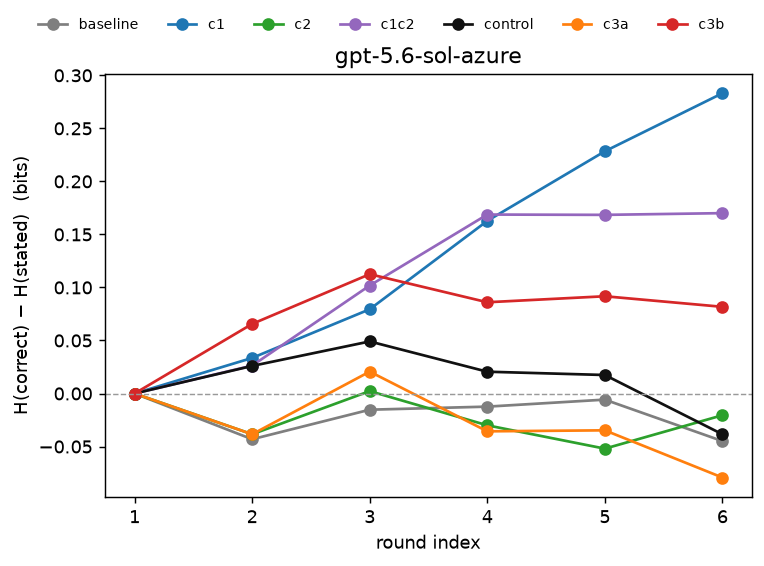
\includegraphics[width=0.62\textwidth]{results/belief_fingerprint_gpt56_azure.png}
\caption{same trajectory plot on this deployment's data. Included since it costs nothing beyond what produced Table D2 above, not because this directional appendix requires its own figure.}
\label{fig:4companion}
\end{figure}

This figure was re-rendered with the shared arm-color/legend styling used elsewhere in this report; the underlying numbers are unchanged from the original run.

On cost, this axis spent 2,117,450 input / 142,744 output tokens across all 7 arms at \texttt{N=29}, priced at GPT-5.6 Sol's published Azure AI Foundry rate (\$5.00/\$30.00 per M input/output tokens, identical to GPT-5.5's OpenAI-direct rate) {[}3{]}: ≈\$14.87.

\section{E\quad Axis 1: reasoning-on/off and the scaffold-mechanism cross (GPT-5.6 Sol, Azure)}\label{e-axis-1-reasoning-onoff-and-the-scaffold-mechanism-cross-gpt-5.6-sol-azure}

Axis 1 asks whether a model's own native reasoning subsumes the external scaffold: a full 6-arm cross (baseline, +C1, +C2, +C1+C2, +C3a, +C3b), each re-run with hidden reasoning (\texttt{reasoning\_effort=\textquotesingle{}medium\textquotesingle{}}, \texttt{temperature=1}, since this deployment's reasoning mode rejects \texttt{temperature=0} {[}2{]}) on GPT-5.6 Sol (Azure AI Foundry, Tier 1, Japan East), compared against the same arms' reasoning-off results (Appendix D). Formalizing the cross at the level of each individual scaffold mechanism, rather than the scaffold as a whole, asks whether native reasoning substitutes for, remediates, or complements each one separately. The token-matched control is excluded on structural grounds: a reasoning-on control column is uninterpretable, since hidden reasoning tokens void the token-matching that defines it.

Everything here is directional signal only: a different, non-same-pass measurement regime, not determinism-frozen, not token-matched, not part of the frozen matrix, and it does not reopen the frontier-model decision (§2.6). It also inherits the known reproducibility gap already documented for this deployment (Appendix D): no dated snapshot, \texttt{system\_fingerprint} not populated on any call. \texttt{reasoning\_effort=\textquotesingle{}medium\textquotesingle{}} + \texttt{temperature=1} acceptance was confirmed empirically by the first live call under this configuration (\texttt{valid:\ true}, no transport error, real reasoning-token counts), not assumed in advance.

This appendix covers provenance and cost for the reasoning-on/off cross; findings and Table E1 appear in §4.5 as RQ5 (secondary, directional).

This axis cost \$36.56 across the six arms. Cumulative GPT-5.6-Azure spend across the 7-arm ablation (Appendix D) and this axis comes to ≈\$51.43.

\textbf{Table E1: Reasoning-OFF vs.~reasoning-ON, all six arms, GPT-5.6 Sol (Azure), \texttt{N=29}} (full-round ratios/regret, to match Table D1).

{\def\LTcaptype{none} % do not increment counter
\begin{longtable}[]{@{}
  >{\raggedright\arraybackslash}p{(\linewidth - 10\tabcolsep) * \real{0.1972}}
  >{\centering\arraybackslash}p{(\linewidth - 10\tabcolsep) * \real{0.1408}}
  >{\raggedleft\arraybackslash}p{(\linewidth - 10\tabcolsep) * \real{0.1972}}
  >{\raggedleft\arraybackslash}p{(\linewidth - 10\tabcolsep) * \real{0.1408}}
  >{\raggedleft\arraybackslash}p{(\linewidth - 10\tabcolsep) * \real{0.1408}}
  >{\raggedleft\arraybackslash}p{(\linewidth - 10\tabcolsep) * \real{0.1831}}@{}}
\toprule\noalign{}
\begin{minipage}[b]{\linewidth}\raggedright
Arm
\end{minipage} & \begin{minipage}[b]{\linewidth}\centering
Regime
\end{minipage} & \begin{minipage}[b]{\linewidth}\raggedleft
EV-realization ↑
\end{minipage} & \begin{minipage}[b]{\linewidth}\raggedleft
Median ↑
\end{minipage} & \begin{minipage}[b]{\linewidth}\raggedleft
EV regret ↓
\end{minipage} & \begin{minipage}[b]{\linewidth}\raggedleft
Dir. agreement ↑
\end{minipage} \\
\midrule\noalign{}
\endhead
\bottomrule\noalign{}
\endlastfoot
Baseline & OFF & 0.864 & 0.833 & 0.170 & 0.821 \\
Baseline & ON & 0.838 & 0.894 & 0.176 & 0.993 \\
+ C1 & OFF & 0.845 & 0.912 & 0.270 & 0.924 \\
+ C1 & ON & 0.819 & 0.860 & 0.209 & 0.993 \\
+ C2 & OFF & 0.901 & 0.919 & 0.127 & 0.924 \\
+ C2 & ON & 0.797 & 0.860 & 0.216 & 1.000 \\
+ C1 + C2 & OFF & 0.868 & 0.912 & 0.231 & 0.572 \\
+ C1 + C2 & ON & 0.807 & 0.875 & 0.253 & 1.000 \\
+ C3a & OFF & 0.905 & 0.919 & 0.114 & 0.966 \\
+ C3a & ON & 0.777 & 0.895 & 0.235 & 0.993 \\
+ C3b & OFF & 0.853 & 0.842 & 0.214 & 1.000 \\
+ C3b & ON & 0.814 & 0.912 & 0.194 & 1.000 \\
\end{longtable}
}

OFF rows reuse Table D1; ON rows are new. All 1,044 ON-regime decision points across the six arms are valid, 0 invalid, 0 transport errors.

Reasoning-on does not help EV-realization on any arm: it is flat-to-negative across the board, and the drop is largest on the arm that needed it least. Every arm's mean ratio falls under reasoning-on; C3a, the best off-reasoning performer in the entire study (Table D1, 0.905), drops the most, to 0.777.

The directional-agreement collapse (Table D1, C1+C2: 0.572) is absent under reasoning-on, but this should be read cautiously rather than as ``reasoning fixes it.'' Off-reasoning, the collapse is specific to the C1+C2 combination, not belief-carry alone (C1 sits at 0.924 off-reasoning, close to the token-matched control's 0.938). Under reasoning-on, both C1 (0.993) and C1+C2 (1.000) sit at or near ceiling, same as every other arm. Two reasons this is not read as a repair. First, hidden reasoning is a different measurement regime, not the same construct: \texttt{directional\_agreement} under reasoning-on scores an \emph{after-the-hidden-reasoning} stated belief against the action, so a high rate here may reflect the visible belief field being retrofit to an already-decided action, not that the action correctly followed the belief. Second, EV-realization moves the wrong way for this to count as a genuine fix: if reasoning-on actually resolved the belief-carry defect, EV-realization on C1+C2 should improve, not fall (0.868 → 0.807). The more defensible reading is that the different measurement regime suppresses the diagnostic signal this metric is built to detect, rather than resolving the underlying belief-to-action problem.

Action diversity differs sharply between the two regimes, which bears on §4.2. Off-reasoning, Sol plays (wide, 1) on 1437 of 1450 evidence-bearing decisions across the seven arms (99.1\%), as GPT-5.5 does (1442 of 1450). Under reasoning-on it uses eight to nine distinct quotes and plays (wide, 1) on only 31 to 48\% of decisions, with (wide, 3) and (wide, 2) next most common. The constant corner quote is therefore a feature of the reasoning-off, temperature-0 operating point; the reasoning-on regime also changes temperature, so this contrast does not isolate reasoning.

\section{F\quad EV-realization distributions (baseline arm)}\label{f-ev-realization-distributions-baseline-arm}

\begin{figure}[H]
\centering
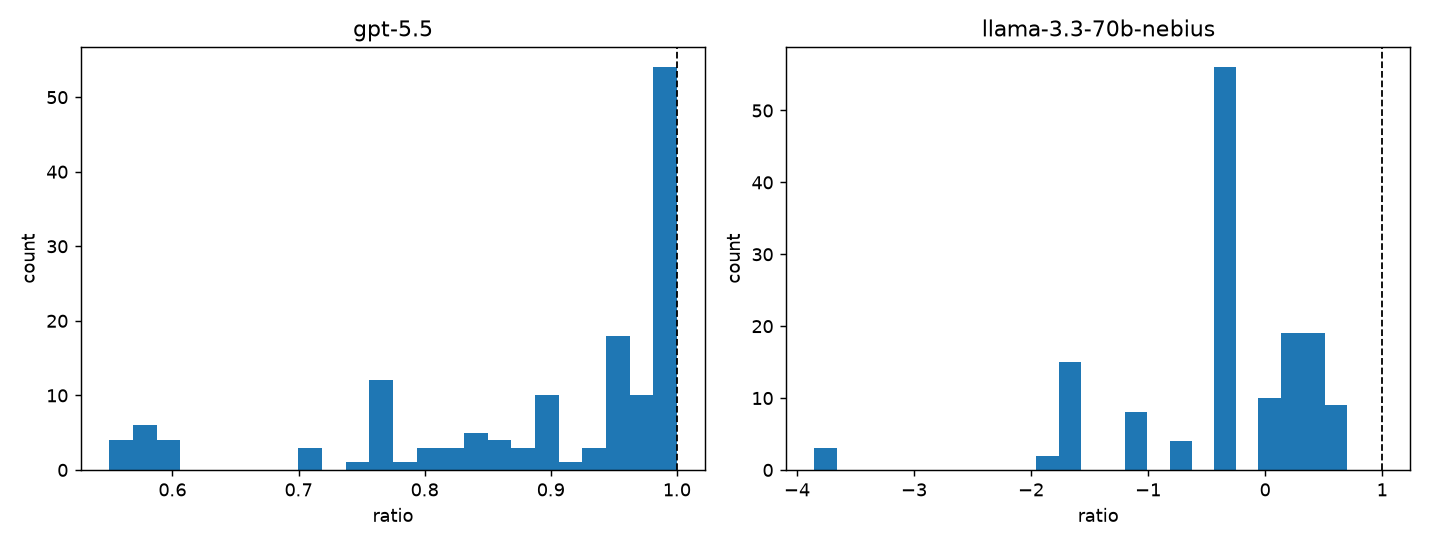
\includegraphics[width=\textwidth]{results/fig3_ev_distributions.png}
\caption{EV-realization ratio distribution, evidence-bearing rounds, baseline arm, one panel per model. The shape behind Table~\ref{tab:1}'s percentiles: the weak model's mass straddling zero rather than one bad tail dragging the mean, against the frontier's near-ceiling concentration.}
\label{fig:2}
\end{figure}

\section{G\quad Cost and efficiency table}\label{g-cost-and-efficiency-table}

\begin{table}[htbp]
\centering
\footnotesize
\caption{Cost and efficiency per arm, relative to the no-scaffold baseline ($N=29$, 174 decisions/arm/model), frontier and weak.}
\label{tab:3}
\begin{tabular}{@{}lrrrrrrr@{}}
\toprule
& \multicolumn{2}{c}{$\Delta$ tokens/round $\downarrow$} & \multicolumn{2}{c}{\$ total, $N=29$ $\downarrow$} & \multicolumn{2}{c}{Latency $\downarrow$} & Quality/1K extra \\
\cmidrule(lr){2-3}\cmidrule(lr){4-5}\cmidrule(lr){6-7}
Arm & Frontier & Weak & Frontier & Weak & Frontier & Weak & tokens (weak) $\uparrow$ \\
\midrule
Baseline & n/a & n/a & \$1.15 & \$0.024 & 1.97s & 3.43s & n/a \\
\;+ C1 & $+216$ & $+220$ & \$1.34 & \$0.030 & 1.86s & 3.43s & 0.35 \\
\;+ C2 & $+1515$ & $+1417$ & \$2.70 & \$0.059 & 3.16s & 6.59s & negative \\
\;+ C1 + C2 & $+1947$ & $+1852$ & \$3.08 & \$0.069 & 3.17s & 6.01s & negative \\
Token-matched control & $+1871$ & $+2503$ & \$4.48 & \$0.115 & 8.35s & 35.5s & 0.04 \\
\;+ C3a & $-46$ & $-45$ & \$1.12 & \$0.023 & 1.65s & 2.79s & free (cost-negative) \\
\;+ C3b & $+195$ & $+197$ & \$1.33 & \$0.029 & 1.62s & 2.32s & \textbf{1.14} \\
\bottomrule
\end{tabular}
\end{table}

\section{H\quad Per-arm values with episode-clustered confidence intervals}\label{h-per-arm-values-with-episode-clustered-confidence-intervals}

Table~\ref{tab:h1} and Table~\ref{tab:h2} give every cell of Table~\ref{tab:2} with episode-clustered 95\% confidence intervals and without rounding, as the meta-review requested. They come from a zero-API replay of the frozen response cache that asserts zero cache misses, and the point estimates reproduce Table 2 to its printed precision. The weak model's EV-realization intervals are wide because the ratio is denominator-unstable there (§4.3). The frontier's decision quality is identical in six arms because its actions are identical (§4.2); the one arm that differs, C3a, plays a different action on 8 of 145 decisions.

\begin{table}[htbp]
\centering
\footnotesize
\caption{GPT-5.5 (frontier). Mean [95\% CI] on evidence-bearing rounds ($N=29$ episodes per arm; 145 decisions), unrounded to three decimals. CIs resample episodes with replacement, 2000 draws, seed 7000.}
\label{tab:h1}
\begin{tabular}{@{}lrrr@{}}
\toprule
Arm & Belief TV distance $\downarrow$ & EV-realization ratio $\uparrow$ & Decision quality $\uparrow$ \\
\midrule
Baseline & 0.063 [0.053, 0.074] & 0.893 [0.862, 0.922] & 0.928 [0.905, 0.947] \\
\;+ C1 (belief-state) & 0.088 [0.075, 0.103] & 0.882 [0.836, 0.924] & 0.928 [0.908, 0.948] \\
\;+ C2 (re-eval loop) & 0.060 [0.053, 0.068] & 0.903 [0.873, 0.929] & 0.928 [0.907, 0.948] \\
\;+ C1 + C2 & 0.082 [0.069, 0.097] & 0.886 [0.845, 0.927] & 0.928 [0.906, 0.949] \\
Token-matched control & 0.052 [0.044, 0.061] & 0.909 [0.877, 0.940] & 0.928 [0.906, 0.948] \\
\;+ C3a & 0.041 [0.038, 0.044] & 0.903 [0.874, 0.929] & 0.927 [0.906, 0.946] \\
\;+ C3b & 0.082 [0.069, 0.096] & 0.928 [0.896, 0.959] & 0.928 [0.907, 0.947] \\
\bottomrule
\end{tabular}
\end{table}

\begin{table}[htbp]
\centering
\footnotesize
\caption{Llama 3.3 70B (weak). Mean [95\% CI] on evidence-bearing rounds ($N=29$ episodes per arm; 145 decisions), unrounded to three decimals. CIs resample episodes with replacement, 2000 draws, seed 7000.}
\label{tab:h2}
\begin{tabular}{@{}lrrr@{}}
\toprule
Arm & Belief TV distance $\downarrow$ & EV-realization ratio $\uparrow$ & Decision quality $\uparrow$ \\
\midrule
Baseline & 0.135 [0.121, 0.150] & $-0.369$ [$-0.565$, $-0.193$] & 0.611 [0.553, 0.666] \\
\;+ C1 (belief-state) & 0.187 [0.153, 0.220] & 0.339 [0.185, 0.477] & 0.687 [0.638, 0.733] \\
\;+ C2 (re-eval loop) & 0.246 [0.220, 0.275] & 0.342 [$-0.175$, 0.907] & 0.073 [0.024, 0.124] \\
\;+ C1 + C2 & 0.283 [0.247, 0.319] & 0.664 [$-0.123$, 2.022] & 0.545 [0.459, 0.626] \\
Token-matched control & 0.117 [0.106, 0.129] & $-0.155$ [$-0.404$, 0.056] & 0.708 [0.650, 0.767] \\
\;+ C3a & 0.111 [0.097, 0.129] & $-0.272$ [$-0.480$, $-0.075$] & 0.667 [0.623, 0.712] \\
\;+ C3b & 0.136 [0.123, 0.151] & $-2.897$ [$-4.857$, $-1.287$] & 0.835 [0.810, 0.862] \\
\bottomrule
\end{tabular}
\end{table}

\end{document}
